% Options for packages loaded elsewhere
\PassOptionsToPackage{unicode}{hyperref}
\PassOptionsToPackage{hyphens}{url}
%
\documentclass[
]{book}
\usepackage{amsmath,amssymb}
\usepackage{lmodern}
\usepackage{ifxetex,ifluatex}
\ifnum 0\ifxetex 1\fi\ifluatex 1\fi=0 % if pdftex
  \usepackage[T1]{fontenc}
  \usepackage[utf8]{inputenc}
  \usepackage{textcomp} % provide euro and other symbols
\else % if luatex or xetex
  \usepackage{unicode-math}
  \defaultfontfeatures{Scale=MatchLowercase}
  \defaultfontfeatures[\rmfamily]{Ligatures=TeX,Scale=1}
\fi
% Use upquote if available, for straight quotes in verbatim environments
\IfFileExists{upquote.sty}{\usepackage{upquote}}{}
\IfFileExists{microtype.sty}{% use microtype if available
  \usepackage[]{microtype}
  \UseMicrotypeSet[protrusion]{basicmath} % disable protrusion for tt fonts
}{}
\makeatletter
\@ifundefined{KOMAClassName}{% if non-KOMA class
  \IfFileExists{parskip.sty}{%
    \usepackage{parskip}
  }{% else
    \setlength{\parindent}{0pt}
    \setlength{\parskip}{6pt plus 2pt minus 1pt}}
}{% if KOMA class
  \KOMAoptions{parskip=half}}
\makeatother
\usepackage{xcolor}
\IfFileExists{xurl.sty}{\usepackage{xurl}}{} % add URL line breaks if available
\IfFileExists{bookmark.sty}{\usepackage{bookmark}}{\usepackage{hyperref}}
\hypersetup{
  pdftitle={Pmetrics User Manual},
  pdfauthor={LAPKB},
  hidelinks,
  pdfcreator={LaTeX via pandoc}}
\urlstyle{same} % disable monospaced font for URLs
\usepackage{color}
\usepackage{fancyvrb}
\newcommand{\VerbBar}{|}
\newcommand{\VERB}{\Verb[commandchars=\\\{\}]}
\DefineVerbatimEnvironment{Highlighting}{Verbatim}{commandchars=\\\{\}}
% Add ',fontsize=\small' for more characters per line
\usepackage{framed}
\definecolor{shadecolor}{RGB}{248,248,248}
\newenvironment{Shaded}{\begin{snugshade}}{\end{snugshade}}
\newcommand{\AlertTok}[1]{\textcolor[rgb]{0.94,0.16,0.16}{#1}}
\newcommand{\AnnotationTok}[1]{\textcolor[rgb]{0.56,0.35,0.01}{\textbf{\textit{#1}}}}
\newcommand{\AttributeTok}[1]{\textcolor[rgb]{0.77,0.63,0.00}{#1}}
\newcommand{\BaseNTok}[1]{\textcolor[rgb]{0.00,0.00,0.81}{#1}}
\newcommand{\BuiltInTok}[1]{#1}
\newcommand{\CharTok}[1]{\textcolor[rgb]{0.31,0.60,0.02}{#1}}
\newcommand{\CommentTok}[1]{\textcolor[rgb]{0.56,0.35,0.01}{\textit{#1}}}
\newcommand{\CommentVarTok}[1]{\textcolor[rgb]{0.56,0.35,0.01}{\textbf{\textit{#1}}}}
\newcommand{\ConstantTok}[1]{\textcolor[rgb]{0.00,0.00,0.00}{#1}}
\newcommand{\ControlFlowTok}[1]{\textcolor[rgb]{0.13,0.29,0.53}{\textbf{#1}}}
\newcommand{\DataTypeTok}[1]{\textcolor[rgb]{0.13,0.29,0.53}{#1}}
\newcommand{\DecValTok}[1]{\textcolor[rgb]{0.00,0.00,0.81}{#1}}
\newcommand{\DocumentationTok}[1]{\textcolor[rgb]{0.56,0.35,0.01}{\textbf{\textit{#1}}}}
\newcommand{\ErrorTok}[1]{\textcolor[rgb]{0.64,0.00,0.00}{\textbf{#1}}}
\newcommand{\ExtensionTok}[1]{#1}
\newcommand{\FloatTok}[1]{\textcolor[rgb]{0.00,0.00,0.81}{#1}}
\newcommand{\FunctionTok}[1]{\textcolor[rgb]{0.00,0.00,0.00}{#1}}
\newcommand{\ImportTok}[1]{#1}
\newcommand{\InformationTok}[1]{\textcolor[rgb]{0.56,0.35,0.01}{\textbf{\textit{#1}}}}
\newcommand{\KeywordTok}[1]{\textcolor[rgb]{0.13,0.29,0.53}{\textbf{#1}}}
\newcommand{\NormalTok}[1]{#1}
\newcommand{\OperatorTok}[1]{\textcolor[rgb]{0.81,0.36,0.00}{\textbf{#1}}}
\newcommand{\OtherTok}[1]{\textcolor[rgb]{0.56,0.35,0.01}{#1}}
\newcommand{\PreprocessorTok}[1]{\textcolor[rgb]{0.56,0.35,0.01}{\textit{#1}}}
\newcommand{\RegionMarkerTok}[1]{#1}
\newcommand{\SpecialCharTok}[1]{\textcolor[rgb]{0.00,0.00,0.00}{#1}}
\newcommand{\SpecialStringTok}[1]{\textcolor[rgb]{0.31,0.60,0.02}{#1}}
\newcommand{\StringTok}[1]{\textcolor[rgb]{0.31,0.60,0.02}{#1}}
\newcommand{\VariableTok}[1]{\textcolor[rgb]{0.00,0.00,0.00}{#1}}
\newcommand{\VerbatimStringTok}[1]{\textcolor[rgb]{0.31,0.60,0.02}{#1}}
\newcommand{\WarningTok}[1]{\textcolor[rgb]{0.56,0.35,0.01}{\textbf{\textit{#1}}}}
\usepackage{longtable,booktabs,array}
\usepackage{calc} % for calculating minipage widths
% Correct order of tables after \paragraph or \subparagraph
\usepackage{etoolbox}
\makeatletter
\patchcmd\longtable{\par}{\if@noskipsec\mbox{}\fi\par}{}{}
\makeatother
% Allow footnotes in longtable head/foot
\IfFileExists{footnotehyper.sty}{\usepackage{footnotehyper}}{\usepackage{footnote}}
\makesavenoteenv{longtable}
\usepackage{graphicx}
\makeatletter
\def\maxwidth{\ifdim\Gin@nat@width>\linewidth\linewidth\else\Gin@nat@width\fi}
\def\maxheight{\ifdim\Gin@nat@height>\textheight\textheight\else\Gin@nat@height\fi}
\makeatother
% Scale images if necessary, so that they will not overflow the page
% margins by default, and it is still possible to overwrite the defaults
% using explicit options in \includegraphics[width, height, ...]{}
\setkeys{Gin}{width=\maxwidth,height=\maxheight,keepaspectratio}
% Set default figure placement to htbp
\makeatletter
\def\fps@figure{htbp}
\makeatother
\setlength{\emergencystretch}{3em} % prevent overfull lines
\providecommand{\tightlist}{%
  \setlength{\itemsep}{0pt}\setlength{\parskip}{0pt}}
\setcounter{secnumdepth}{5}
\usepackage{booktabs}
\ifluatex
  \usepackage{selnolig}  % disable illegal ligatures
\fi
\usepackage[]{natbib}
\bibliographystyle{plainnat}

\title{Pmetrics User Manual}
\author{LAPKB}
\date{2022-02-18}

\begin{document}
\maketitle

{
\setcounter{tocdepth}{1}
\tableofcontents
}
\hypertarget{preface}{%
\chapter{Preface}\label{preface}}

This is the manual for Pmetrics, a population modeling and simulation package for R.

Pmetrics is the result of years of labor from many people. It was created by the Laboratory of Applied Pharmacokinetics and Bioinformatics (LAPKB).

\hypertarget{a-brief-history}{%
\section{A brief history}\label{a-brief-history}}

LAPKB, established in 1973 as LAPK by Roger Jelliffe, MD, has been continually associated with the University of Southern California and the USC Keck School of Medicine. Since 2012, it has been housed under the Saban Research Institute at Children's Hospital Los Angeles (CHLA).

Since its inception, LAPKB has been a pharmacometric resource for optimal study and control of pharmacokinetic/pharmacodynamic systems and for individualized drug therapy and personalized medicine. It has been continually supported by grants, including from The National Institute for General Medical Studies (NIGMS), National Institute of Biomedical Imagining and Bioengineering (NIBIB), the Eunice Kennedy Shriver National Institute of Child Health and Human Development (NICHD), the US Food and Drug Administration (FDA), and by the Stella Slutzky Kunin Memorial Research Fund.

The laboratory has employed physicians, pharmacists, engineers, statisticians, and mathematicians. LAPKB has special strengths in nonparametric statistical methods, optimal stochastic control, optimal design of pharmacokinetic experiments and clinical trials, and practical application of tools for optimal clinical therapy.

The laboratory also seeks collaborative relationships to further the understanding and development of this field of Clinical Pharmacology. These collaborations may take the form of clinical trials and evaluations of therapeutic methods or of development and software implementation of new concepts. Educational opportunities in the form of workshops and visiting scholars are available to physicians, pharmacists, engineers, mathematicians, and other investigators.

\hypertarget{people}{%
\section{People}\label{people}}

This is not an exhaustive list by any means, but highlights some individuals who have made exceptional contributions to the lab.

\begin{itemize}
\tightlist
\item
  Roger Jellife, MD - founder and pioneer. Passed away June 22, 2002.
\item
  Alan Schumitzky, PhD - Emeritus Professor of Mathematics at USC. Professor Schumitzky's research interests are focused on estimation and control theory, applied pharmacokinetics, complex analysis, and software development. He developed NPEM, co-developed NPAG, NPOD, and every other algorithm from the lab, and he continues to share his genius.
\item
  Robert Leary, PhD - co-developer of NPAG and former consultant to the lab.
\item
  David Bayard, PhD - consultant to the lab and expert in optimal control. He developed the Multiple Model algorithm powering BestDose, as well as the MMopt optimal sampling algorithm.
\item
  Michael van Guilder PhD - consultant to the lab who turned all of the ideas into working, stable, reliable Fortran code.
\item
  Walter Yamada, PhD - Current scientific programmer, modeler, and the person who knows the code the best and manages the lab on a daily basis. He developed the Poisson likelihood function and makes updates to the code every day.
\item
  Julian Otalvaro - Scientfic programmer who has transformed Pmetrics by developing the R6 framework, moving it to Github, and just about every other aspect of the package. He is also one of the labs experts in machine learning.
\item
  Rong Chen, PhD - post-doc and author of RPEM. He is our expert in Fortran and use of MPI to parallelize code.
\item
  Alona Kryshchenko, PhD - consulant and co-developer of NPOD.
\item
  Michael Neely, MD - current leader of the lab, physician and dabbler in statistics. He wrote all of the original Pmetrics package and continues to write to this day, in addition to all the other jobs associate with Principle Investigator and Chief of the Division of Infectious Diseases at CHLA.
\end{itemize}

\hypertarget{citing-pmetrics}{%
\section{Citing Pmetrics}\label{citing-pmetrics}}

Please help us maintain our funding to provide Pmetrics as a free
research tool to the pharmacometric community. If you use Pmetrics in a
publication, you can cite it as below.

\begin{Shaded}
\begin{Highlighting}[]
\FunctionTok{citation}\NormalTok{(}\StringTok{"Pmetrics"}\NormalTok{)}
\end{Highlighting}
\end{Shaded}

\begin{verbatim}
## 
## To cite package 'Pmetrics' in publications use:
## 
##   Neely MN, van Guilder MG, Yamada WM, Schumitzky A, Jelliffe RW.
##   Accurate detection of outliers and subpopulations with Pmetrics, a
##   nonparametric and parametric pharmacometric modeling and simulation
##   package for R. Therapeutic Drug Monitoring. 2012; 34(4): 467-476.
## 
## A BibTeX entry for LaTeX users is
## 
##   @Article{,
##     title = {Accurate Detection of outliers and subpopulations with Pmetrics: a non-parametric and parametric pharmacometric modeling and simulation package for R},
##     author = {Michael Neely and Michael {van Guilder} and Walter Yamada and Alan Schumitzky and Roger Jelliffe},
##     year = {2012},
##     journal = {Therapeutic Drug Monitoring},
##     volume = {34},
##     number = {4},
##     pages = {467-476},
##   }
\end{verbatim}

\hypertarget{donate}{%
\section{Donate}\label{donate}}

If you appreciate the enormous work to develop and maintain Pmetrics,
please consider a \href{https://www.paypal.com/donate?token=3aF-w2c7Dw35BWYefFIX1QUD9j7Uu2J3KGkmh7vWF_A8ifjKc8E1Bp05NmDCH__6GwB49bXYOp_tKNpw}{donation}.

\hypertarget{introduction}{%
\chapter{Introduction}\label{introduction}}

Thank you for your interest in Pmetrics! This guide provides
instructions and examples to assist users of the Pmetrics R package, by
the Laboratory of Applied Pharmacokinetics and Bioinformatics at the
Saban Research Institute, Children's Hospital Los Angeles, and the
Department of Pediatrics, Keck School of Medicine, University of
Southern California. Please see our website at
\href{http://www.lapk.org}{\underline{http://www.lapk.org}} for more
information.

\hypertarget{r6-architecture}{%
\section{R6 architecture}\label{r6-architecture}}

\textbf{As of v. 2.0}, Pmetrics is shifting to an architecture less dependent on
reading and writing files. Data files are unchanged and described later in
this manual.

Model files can now be defined as an R object, instead of in a text file.
Pmetrics can suppoort legacy runs with the old-style text file models, but
users are encouraged to change to the new methods. Throughout this manual we
will indicate the new style with the {R6} designation to reflect the
object-oriented R6 style of programming available in R that makes it more
consistent with object-oriented languages such as Python. We will indicate
old-style approaches with {Legacy}.

\textbf{Here are some tips for using this guide.}

\begin{itemize}
\item
  The table of contents to the left is expandable and navigable.
\item
  Items that are hyperlinked can be selected to cross reference
  within this manual or link to external sites.
\item
  \texttt{Items} correspond to inline examples of R code, which are not evaluted
  in this document, but serve as templates for what may be typed into your
  R console or script. They may not necessarily be executable if typed verbatim.
\end{itemize}

\hypertarget{disclaimer}{%
\section{Disclaimer}\label{disclaimer}}

You, the user, assume all responsibility for acting on the results
obtained from Pmetrics. The Laboratory of Applied Pharmacokinetics and
Bioinformatics (LAPKB), members and consultants to LAPKB, and Children's
Hospital Los Angeles and the University of Southern California and their
employees assume no liability whatsoever. Your use of the package
constitutes your agreement to this provision.

\hypertarget{system-requirements-and-installation}{%
\section{System Requirements and Installation}\label{system-requirements-and-installation}}

Pmetrics and all required components will run under Mac (Unix), Windows,
and Linux. There are three \emph{required} software components
which must be installed on your system \textbf{in this order}:

\begin{enumerate}
\def\labelenumi{\arabic{enumi}.}
\item
  The statistical programming language and environment ``\textbf{R}''

  \begin{itemize}
  \tightlist
  \item
    After installing R, we highly recommended that you also install
    \textbf{Rstudio}, a user-friendly environment for R.
  \end{itemize}
\item
  The \textbf{Pmetrics} package for R
\item
  The \textbf{gfortran} Fortran compiler.
\end{enumerate}

All components have versions for Mac, Windows, and Linux environments,
and 64- bit processors. Systems with 32-bit processors are no longer
supported. All are free of charge.

\hypertarget{r}{%
\subsubsection{R}\label{r}}

R is a free software environment for statistical computing and graphics,
which can be obtained from
\href{http://www.R-project.org}{\underline{http://www.R-project.org}}.
Pmetrics is a library for R.

\hypertarget{rstudio}{%
\subsubsection{Rstudio}\label{rstudio}}

We strongly recommend using \href{http://rstudio.org/}{Rstudio} rather than any
other R interface.

\hypertarget{pmetrics}{%
\subsubsection{Pmetrics}\label{pmetrics}}

If you are reading this manual, then you have likely visited our website
at \href{http://www.lapk.org}{\underline{http://www.lapk.org}}, where you
can select the software tab to access instructions.
As of version 1.9, Pmetrics is distributed on github and is a self-contained
package that will install gfortran with your permission, if it is not
already installed on your computer. Installing from github will also install
all packages upon which Pmetrics depends.

\hypertarget{gfortran}{%
\subsubsection{Gfortran}\label{gfortran}}

In order to run Pmetrics, a Fortran compiler compiler is required.
Pmetrics is designed to work with gfortran, a free compiler. After you
have installed Pmetrics, it will check your system for an active
gfortran installation. If it doesn't find one, it will offer to download
and install it. From there, installation should proceed automatically.
This is by far the easiest and most reliable way to complete
installation. Rest assured that no files are installed without your
permission.

If you do not wish to do this, you will have to get components manually,
and the first command to run is \texttt{PMbuild()}. You can get detailed
instructions on how to obtain and install gfortran appropriate for your
system on our \href{http://www.lapk.org/Pmetrics_install_manual.php}{LAPKB website}.

\hypertarget{what-this-manual-is-not}{%
\section{What This Manual Is Not}\label{what-this-manual-is-not}}

We assume that the user has familiarity with population modeling and R,
and thus this manual is not a tutorial for basic concepts and techniques
in either domain. We have tried to make the R code simple, regular and
well documented. A very good free online resource for learning the
basics of R can be found at \href{http://www.statmethods.net/index.html}{Stat Methods}.

We recognize that initial use of a new software package can be complex,
so please feel free to contact us at any time, preferably through the
\href{http:/www.lapk.org}{Pmetrics forum} or directly by \href{mailto:contact@lapk.org}{email}.

This manual is also not intended to be a theoretical treatise on the
algorithms used in IT2B or NPAG. For that, the user is directed to our
\href{http://www.lapk.org}{website}.

\hypertarget{getting-help-and-updates}{%
\section{Getting Help and Updates}\label{getting-help-and-updates}}

Within R, you can use
\texttt{help("command")} or \texttt{?command} in the R console to see detailed help files
for any Pmetrics command. Many commands have examples included in this
documentation and you can execute the examples with \texttt{example(command)}.

Pmetrics will check for updates automatically every time you load it
with \texttt{library(Pmetrics)} and you are connected to the internet.
If an update is available, it will provide a
brief message to inform you. You can then reinstall the package from github.

\hypertarget{customizing-pmetrics-options}{%
\section{Customizing Pmetrics Options}\label{customizing-pmetrics-options}}

You can change global options in Pmetrics with
\texttt{setPMoptions(sep,\ dec,server\textbackslash{}\_address)}.

Currently you can change three options: \texttt{sep} and \texttt{dec} will allow Pmetrics
to read data files whose field separators are semicolons and decimal
separators are commas, e.g.~\texttt{setPMoptions(sep=";",\ dec=",")}. These
options will persist from session to session until changed. The third
option, \texttt{server\textbackslash{}\_address}, allows you to specify the address of a remote
server with Pmetrics installed, to allow remote runs.

\texttt{getPMoptions()} will return the current options.

\hypertarget{pmetrics-overview}{%
\chapter{Pmetrics Overview}\label{pmetrics-overview}}

\hypertarget{software-engines}{%
\section{Software engines}\label{software-engines}}

There are three main software engines that Pmetrics controls.

\begin{itemize}
\item
  \textbf{IT2B} is the ITerative 2-stage Bayesian parametric population PK modeling
  program. It is generally used to estimate parameter ranges to pass to
  NPAG. It will estimate values for population model parameters under the
  assumption that the underlying distributions of those values are normal
  or transformed to normal.
\item
  \textbf{NPAG} is the Non-parametric Adaptive Grid software. It will create a
  non-parametric population model consisting of discrete support points,
  each with a set of estimates for all parameters in the model plus an
  associated probability (weight) of that set of estimates. There can be
  at most one point for each subject in the study population. There is no
  need for any assumption about the underlying distribution of model
  parameter values.
\item
  The \textbf{Simulator} is a semi-parametric Monte Carlo simulation software
  program that can use the output of IT2B or NPAG to build randomly
  generated response profiles (e.g.~time-concentration curves) for a given
  population model, parameter estimates, and data input. Simulation from a
  non-parametric joint density model, i.e.~NPAG output, is possible, with
  each point serving as the mean of a multivariate normal distribution,
  weighted according to the weight of the point. The covariance matrix of
  the entire set of support points is divided equally among the points for
  the purposes of simulation.
\end{itemize}

\hypertarget{pmetrics-control-functions}{%
\section{Pmetrics control functions}\label{pmetrics-control-functions}}

{R6}

Pmetrics uses \texttt{PM\_model} to create model objects and \texttt{PM\_fit} to create
objects that combine the model with the data, ready to be run (fitted),
generating probability distributions for primary model parameters.

These functions replace the following Legacy functions: \texttt{ITrun}, \texttt{ERRrun},
\texttt{NPrun}.

\texttt{PMload} is aliased as \texttt{PM\_load} for consistency with the above functions.
Similar to the Legacy version, it loads the results of a run into R to be
accessible to the user for analysis, plotting, etc. Different from the Legacy
version, it loads the results into another R6 object, \texttt{PM\_result} instead of
the current environment.

Invoking the simulator in R6 is unchanged, i.e.~use \texttt{SIMrun}.

{Legacy}

Pmetrics has groups of R functions named logically to run each of these
programs and to extract the output. Again, these are extensively
documented within R by using the \texttt{help(command)} or \texttt{?command\ syntax}.

\begin{itemize}
\item
  \texttt{ITrun}, \texttt{ITparse}, \texttt{ERRrun}
\item
  \texttt{NPrun}, \texttt{NPparse}
\item
  \texttt{PMload}, \texttt{PMsave}, \texttt{PMreport}
\item
  \texttt{SIMrun}, \texttt{SIMparse}
\end{itemize}

\hypertarget{run-functions}{%
\subsection{Run functions}\label{run-functions}}

{R6}

Once a \texttt{PM\_fit} object is created, which combines a model with a data file,
it can be run by using the syntax \texttt{\$run()} to access the appropriate function
defined for the \texttt{PM\_fit} object.

\begin{Shaded}
\begin{Highlighting}[]
\NormalTok{run1 }\OtherTok{\textless{}{-}} \FunctionTok{PM\_fit}\NormalTok{(model,data)}
\NormalTok{run1}\SpecialCharTok{$}\FunctionTok{run}\NormalTok{(options)}
\end{Highlighting}
\end{Shaded}

{R6} {Legacy}

For IT2B and NPAG, the ``run'' functions generate batch files, which when
executed, launch the software programs to do the analysis. \texttt{\$run(engine="err")}
or \texttt{ERRrun()} is a special implementation of IT2B designed to estimate
the assay error polynomial coefficients from the data, when they cannot be calculated from assay validation data (using \texttt{makeErrorPoly()}) supplied by the
analytical laboratory. The batch files contain all the information
necessary to complete a run, tidy the output into a date/time stamped
directory with meaningful subdirectories, extract the information,
generate a report, and a saved Rdata file of parsed output which can be
quickly and easily loaded into R. On Mac (Unix) and Linux systems,
the batch file automatically launches in a Terminal window.
Prior to v1.9, on Windows systems, the batch file was launched manually,
but as of v1.9, this manual step is no longer necessary. The execution of
the program to do the actual model parameter estimation is independent
of R, so that the user is free to use R for other purposes.

For the Simulator, the \texttt{SIMrun} function will execute the program
directly within R.

\hypertarget{parse-functions}{%
\subsection{Parse functions}\label{parse-functions}}

{R6} {Legacy}

For all programs, the ``parse'' functions will extract the primary output
from the program into meaningful R data objects. For IT2B and NPAG, this
is done automatically at the end of a successful run, and the objects
are saved in the output subdirectory as IT2Bout.Rdata or NPAGout.Rdata,
respectively. These functions generally run automatically and are not
necessary for the user to access.

\hypertarget{saving-and-loading-functions}{%
\subsection{Saving and loading functions}\label{saving-and-loading-functions}}

{R6}

After a successful IT2B or NPAG run, \texttt{PMload} or \texttt{PM\_load} creates a
\texttt{PM\_result} object rather than loading run results into the current
environment and suffixed with the run number.

\begin{Shaded}
\begin{Highlighting}[]
\NormalTok{fit1 }\OtherTok{\textless{}{-}} \FunctionTok{PM\_load}\NormalTok{(}\DecValTok{1}\NormalTok{)}
\FunctionTok{plot}\NormalTok{(fit1}\SpecialCharTok{$}\NormalTok{op)}
\end{Highlighting}
\end{Shaded}

{Legacy}

For IT2B and NPAG, the \texttt{PM\_load} function can be used to load either
of the above .Rdata files after a successful run. Objects will be loaded
into the current environment in R and suffixed with ``.run'', where ``run'' is
the run number.

\begin{Shaded}
\begin{Highlighting}[]
\FunctionTok{PM\_load}\NormalTok{(}\DecValTok{1}\NormalTok{)}
\FunctionTok{plot}\NormalTok{(op}\FloatTok{.1}\NormalTok{)}
\end{Highlighting}
\end{Shaded}

{Update}
\texttt{PMsave} is the
companion to \texttt{PMload} and can re-save modified objects to the .Rdata file.

\hypertarget{report-generation}{%
\subsection{Report generation}\label{report-generation}}

{R6} {Legacy}

The \texttt{PMreport} function is automatically run at the end of a successful
NPAG and IT2B run, and it will generate an HTML page with summaries of
the run, as well as the .Rdata files and other objects. The default
browser will be automatically launched for viewing of the HTML report
page. See the \protect\hyperlink{outputs}{Pmetrics
Outputs} section.

\hypertarget{data-manipulation-functions}{%
\section{Data manipulation functions}\label{data-manipulation-functions}}

{R6} {Legacy}

Within Pmetrics there are also functions to manipulate data .csv files
and process and plot extracted data.

\begin{itemize}
\item
  Manipulate data .csv files: \texttt{PMreadMatrix}, \texttt{PMcheck}, \texttt{PMwriteMatrix},
  \texttt{PMmatrixRelTime}, \texttt{PMwrk2csv}, \texttt{NM2PM}, \texttt{PMmb2csv}
\item
  Process data: \texttt{makeAUC}, \texttt{makeCov}, \texttt{makeCycle}, \texttt{makeFinal}, \texttt{makeOP}, \texttt{makePTA},
  \texttt{makeErrorPoly}
\item
  Plot data: \texttt{plot.PMcov}, \texttt{plot.PMcycle}, \texttt{plot.PMfinal}, \texttt{plot.PMmatrix},
  \texttt{plot.PMop},\texttt{plot.PMsim}, \texttt{plot.PMvalid}, \texttt{plot.PMpta}
\item
  Model selection and diagnostics: \texttt{PMcompare}, \texttt{plot.PMop} (with residual
  option), \texttt{makeValid}, \texttt{plot.PMvalid}, \texttt{PMstep}
\item
  Pmetrics function defaults: \texttt{setPMoptions}, \texttt{getPMoptions}
\end{itemize}

Again, all functions have extensive help files and examples which can be
examined in R by using the \texttt{help(command)} or \texttt{?command} syntax.

\hypertarget{general-workflow}{%
\chapter{General Workflow}\label{general-workflow}}

{R6}

The general Pmetrics workflow in R6 for IT2B and NPAG is shown in the
following diagram.

The user supplies the items in \textbf{yellow}. R is used to specify the working directory containing the data .csv file. The model file is created in R using
the \texttt{PM\_model} function. When combined using \texttt{PM\_fit} and the \texttt{\$run()} function
on the resulting object, a batch file is generated by R, causing the preparation
program to be compiled and executed. An instruction file is generated
automatically by the contents of the data and model, and by
arguments to the \texttt{\$run()} function. The batch file
will then compile and execute the engine file according to the
instructions, which will generate several output files upon completion.
Finally, the batch file will call the R script to generate the summary
report and several data objects, including the IT2Bout.Rdata or
NPAGout.Rdata files which can be loaded into R subsequently using
\texttt{PM\_load}. Objects that are modified can be saved back to the .Rdata
files with \texttt{PMsave}.

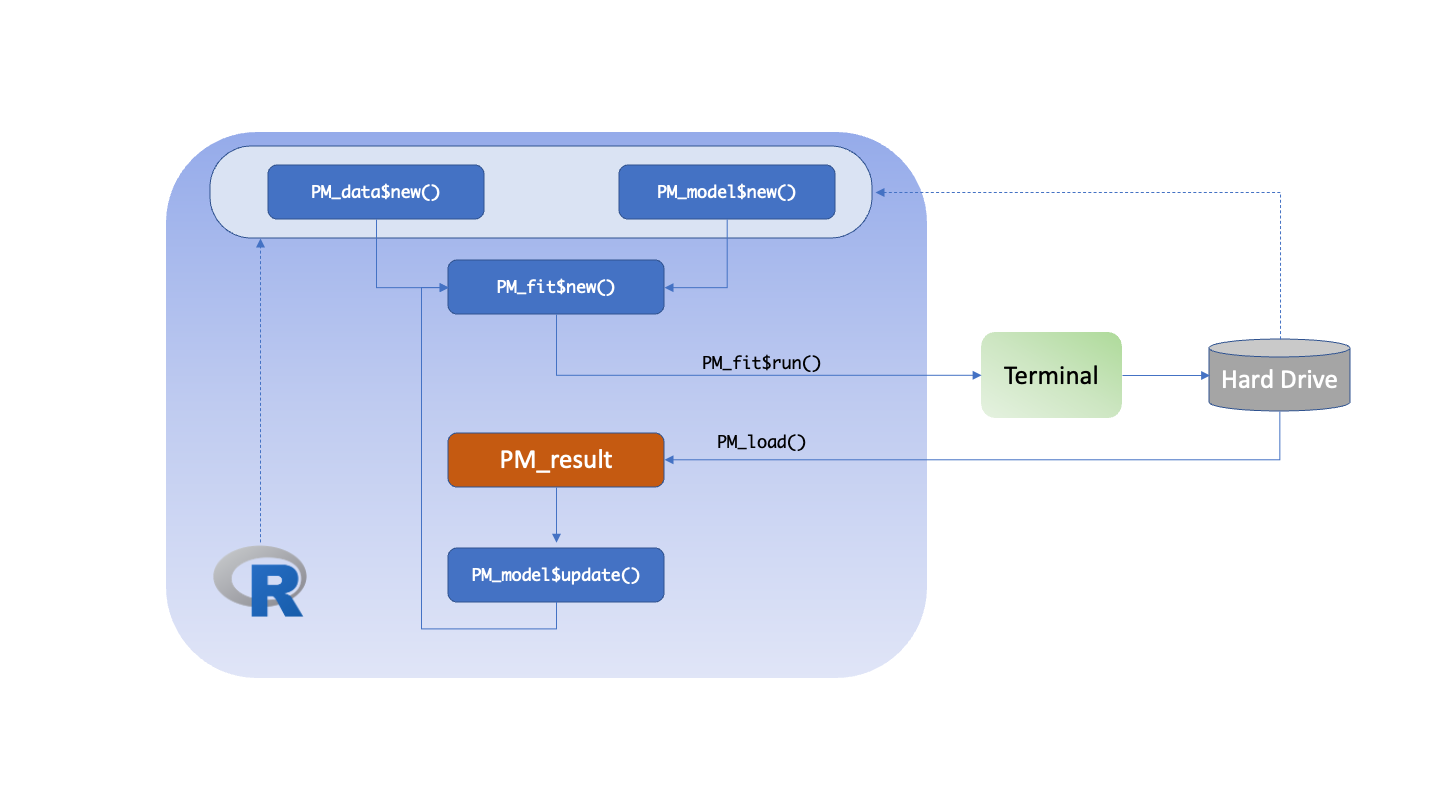
\includegraphics{Images/Slide1.png}

{Legacy}

The general Pmetrics workflow in Legacy for IT2B and NPAG is shown in the
following diagram. The major differences compared to R6 are that the model is a text file, and the commands to start the run are different.

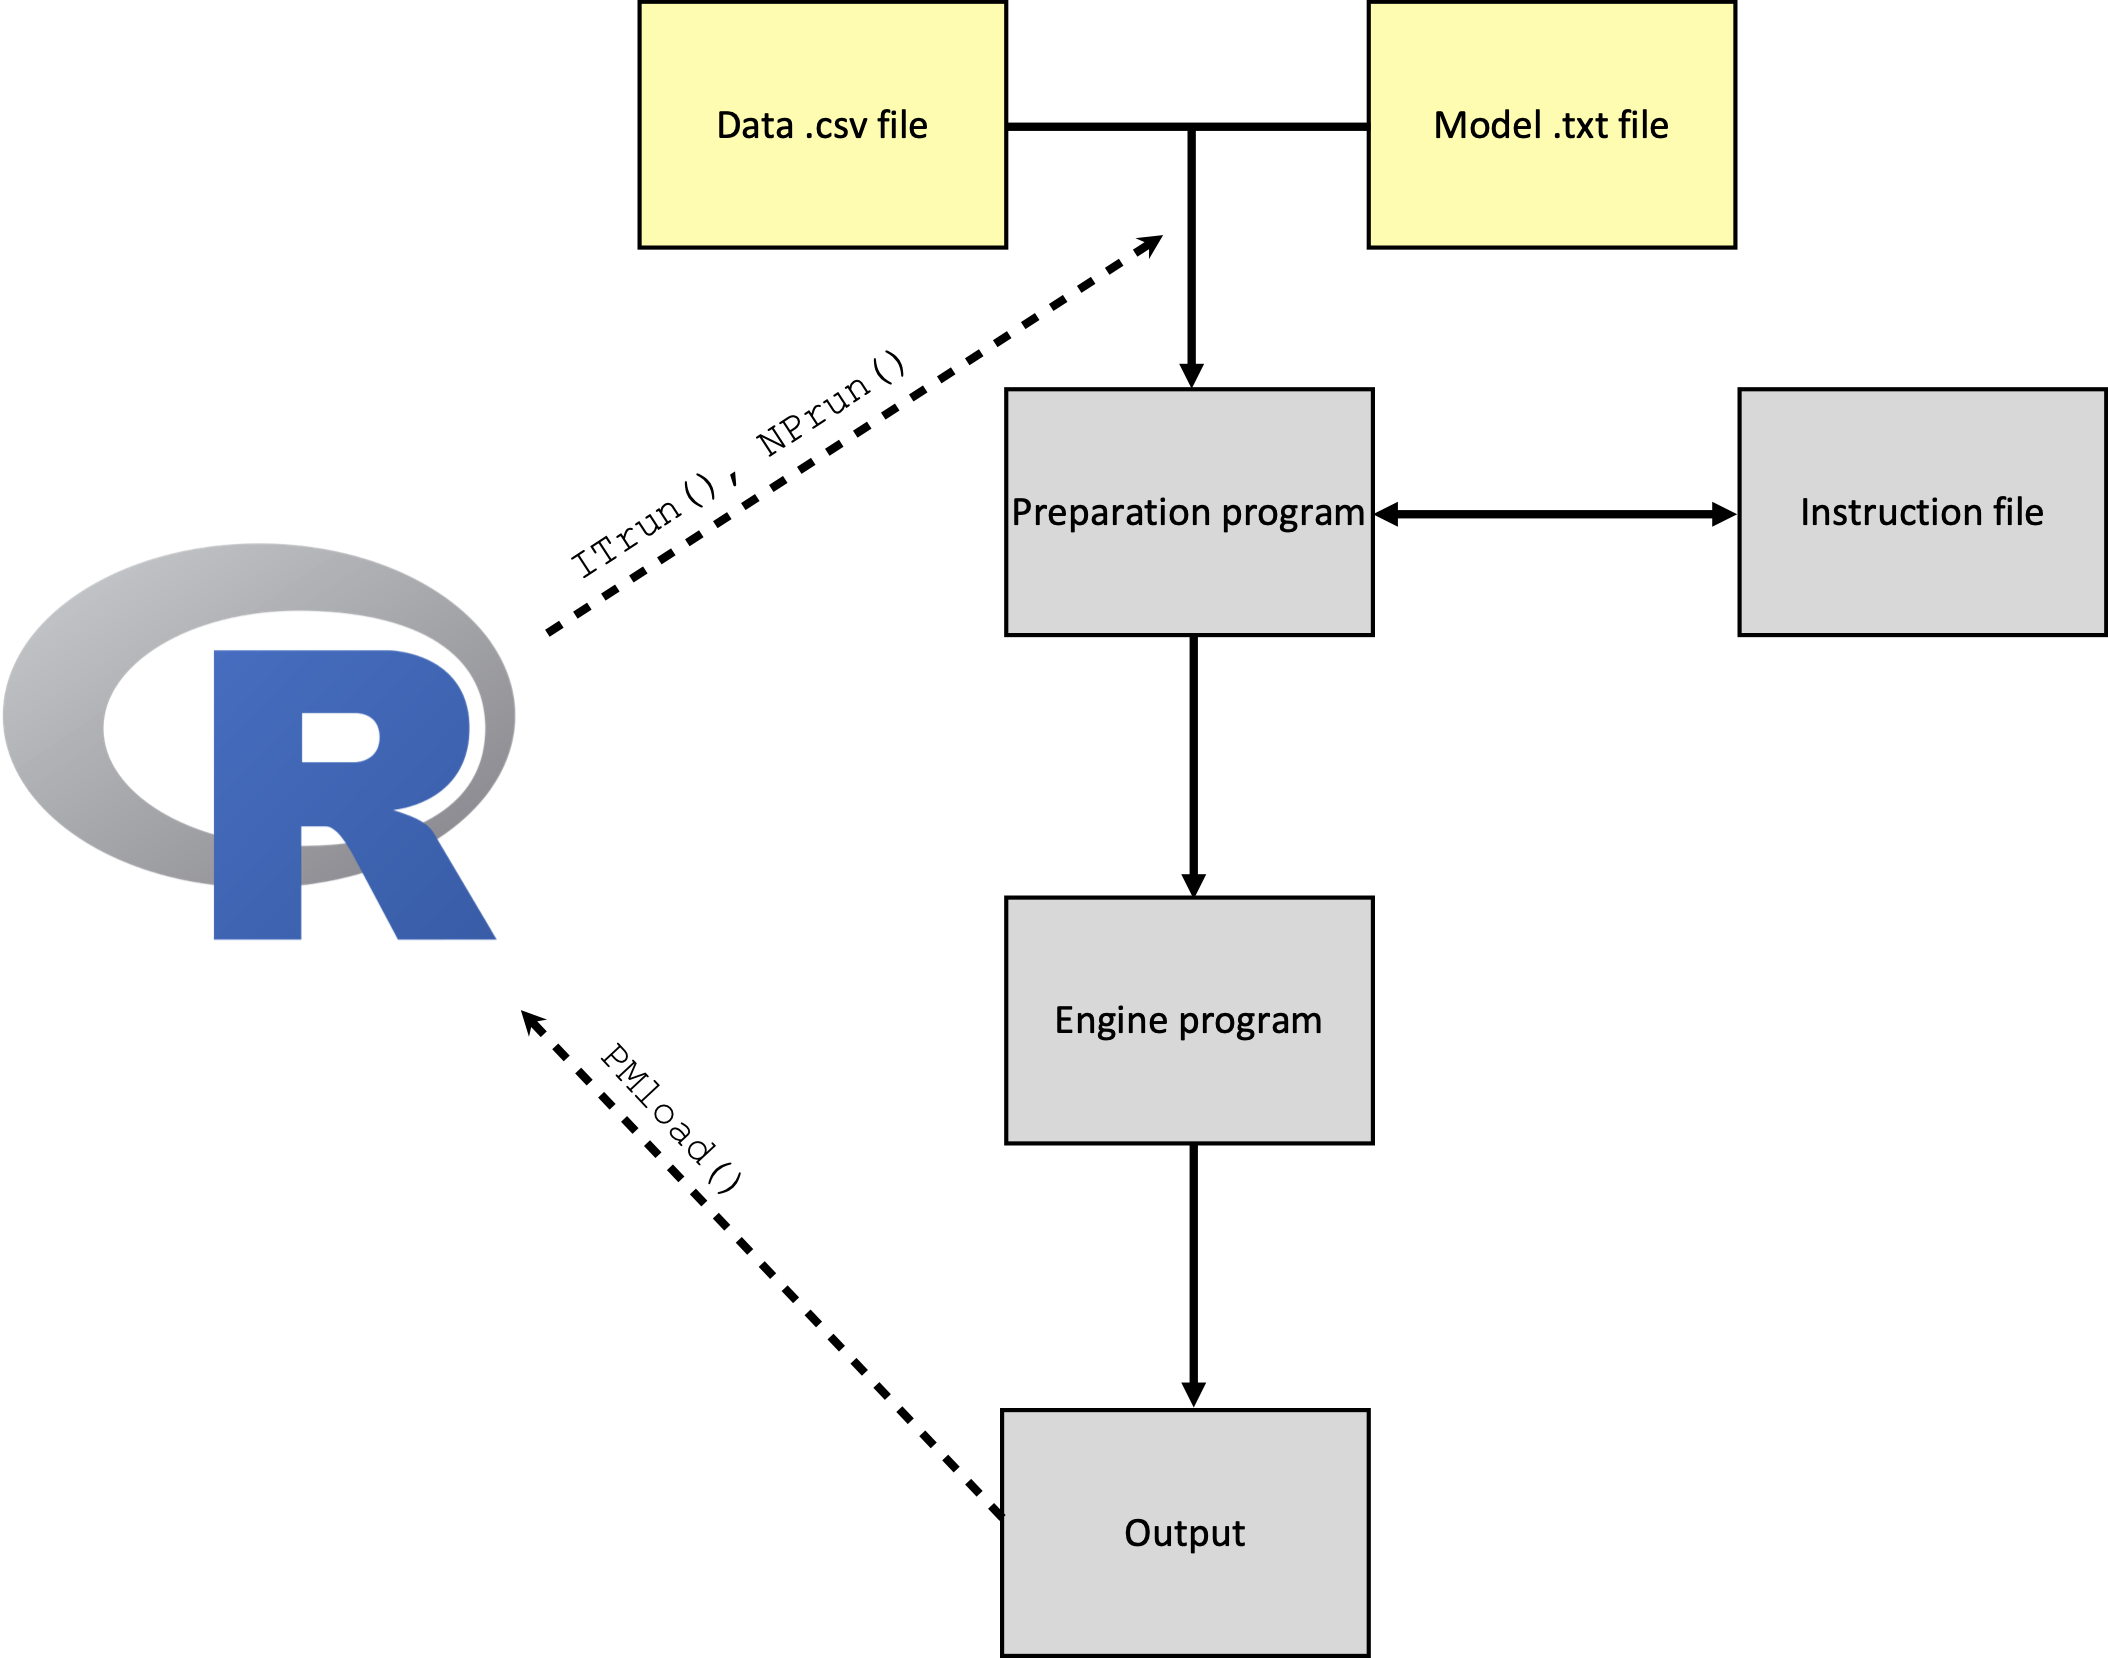
\includegraphics{Images/Slide2.png}

The user supplies the items in \textbf{yellow} as arguments to
the run functions. R is used to specify the working directory containing the data.csv and
model.txt files. Through the batch file generated by R, the preparation
program is compiled and executed. The instruction file is generated
automatically by the contents of the data and model files, and by
arguments to the \texttt{NPrun}, \texttt{ITrun} or \texttt{ERRrun} commands. The batch file
will then compile and execute the engine file according to the
instructions, which will generate several output files upon completion.
Finally, the batch file will call the R script to generate the summary
report and several data objects, including the IT2Bout.Rdata or
NPAGout.Rdata files which can be loaded into R subsequently using
\texttt{PMload}. Objects that are modified can be saved back to the .Rdata
files with \texttt{PMsave}.

Both input files (data, model) are text files which can be edited
directly.

\hypertarget{pmetrics-input-files}{%
\chapter{Pmetrics Input Files}\label{pmetrics-input-files}}

\hypertarget{data.csv-files}{%
\section{Data.csv Files}\label{data.csv-files}}

Pmetrics accepts input as a spreadsheet ``matrix'' format. It is designed
for input of multiple records in a concise way. \textbf{Please keep the number
of characters in the file name ≤ 8.}

\hypertarget{data-file-format}{%
\subsection{Data file format}\label{data-file-format}}

Files are in comma-separated-values (.csv) format. Examples of programs
that can save .csv files are any text editor (e.g.~TextEdit on Mac,
Notepad on Windows) or spreadsheet program (e.g.~Excel). Click on
hyperlinked items to see an explanation.

\textbf{IMPORTANT}: The order, capitalization and names of the header and the
first 12 columns are fixed. All entries must be numeric, with the
exception of ID and ``.'' for non-required placeholder entries.

\textbf{\emph{POPDATA DEC\_11}}

\begin{tabular}{l|r|r|r|r|r|r|r|l|r|r|r|r|r|r}
\hline
\#ID & EVID & TIME & DUR & DOSE & ADDL & II & INPUT & OUT & OUTEQ & C0 & C1 & C2 & C3 & COV\\
\hline
GH & 1 & 0.00 & 0.0 & 400 & . & . & 1 & . & . & . & . & . & . & 10.0\\
\hline
GH & 0 & 0.50 & . & . & . & . & . & 0.42 & 1 & . & . & . & . & .\\
\hline
GH & 0 & 1.00 & . & . & . & . & . & 0.46 & 1 & . & . & . & . & .\\
\hline
GH & 0 & 2.00 & . & . & . & . & . & 2.47 & 1 & . & . & . & . & .\\
\hline
GH & 4 & 0.00 & 0.0 & 150 & . & . & 1 & . & . & . & . & . & . & .\\
\hline
GH & 1 & 3.50 & 0.5 & 150 & . & . & 1 & . & . & . & . & . & . & .\\
\hline
GH & 0 & 5.12 & . & . & . & . & . & 0.55 & 1 & . & . & . & . & .\\
\hline
GH & 0 & 24.00 & . & . & . & . & . & 0.52 & 1 & . & . & . & . & .\\
\hline
1423 & 1 & 0.00 & 1.0 & 400 & -1 & 12 & 1 & . & . & . & . & . & . & 34.5\\
\hline
1423 & 1 & 0.10 & 0.0 & 100 & . & . & 2 & . & . & . & . & . & . & .\\
\hline
1423 & 0 & 1.00 & . & . & . & . & . & -99 & 1 & 0.01 & 0.1 & 0.00 & 0.000 & .\\
\hline
1423 & 0 & 2.00 & . & . & . & . & . & 0.38 & 1 & 0.01 & 0.1 & 0.00 & 0.000 & .\\
\hline
1423 & 0 & 2.00 & . & . & . & . & . & 1.6 & 2 & 0.05 & 0.2 & -0.11 & 0.002 & .\\
\hline
\end{tabular}

\begin{itemize}
\item
  \textbf{\emph{POPDATA DEC\_11}} This is the fixed header for the file and must be
  in the first line. It identifies the version. It is not the date of your
  data file.
\item
  \textbf{\emph{\#ID}} This field must be preceded by the ``\#'' symbol to confirm
  that this is the header row. It can be numeric or character and
  identifies each individual. All rows must contain an ID, and all
  records from one individual must be contiguous. Any subsequent row
  that begins with ``\#'' will be ignored, which is helpful if you want to
  exclude data from the analysis, but preserve the integrity of the
  original dataset, or to add comment lines. IDs should be 11 characters
  or less but may be any alphanumeric combination. \textbf{There can be at
  most 800 subjects per run.}
\item
  \textbf{\emph{EVID}} This is the event ID field. It can be 0, 1, or 4. Every row
  must have an entry.

  \begin{itemize}
  \item
    0 = observation
  \item
    1 = input (e.g.~dose)
  \item
    2, 3 are currently unused
  \item
    4 = reset, where all compartment values are set to 0 and the time
    counter is reset to 0. This is useful when an individual has multiple
    sampling episodes that are widely spaced in time with no new
    information gathered. This is a dose event, so dose information needs
    to be complete.
  \end{itemize}
\item
  \textbf{\emph{TIME}} This is the elapsed time in decimal hours since the first
  event. It is not clock time (e.g.~09:30), although the \texttt{PMmatrixRelTime}
  function can convert dates and clock times to decimal hours.
  Every row must have an entry, and within a given ID, rows
  must be sorted chronologically, earliest to latest.
\item
  \textbf{\emph{DUR}} This is the duration of an infusion in hours. If EVID=1,
  there must be an entry, otherwise it is ignored. For a bolus (i.e.~an
  oral dose), set the value equal to 0.
\item
  \textbf{\emph{DOSE}} This is the dose amount. If EVID=1, there must be an entry,
  otherwise it is ignored.
\item
  \textbf{\emph{ADDL}} This specifies the number of additional doses to give at
  interval II. It may be missing for dose events (EVID=1 or 4), in which
  case it is assumed to be 0. It is ignored for observation (EVID=0)
  events. Be sure to adjust the time entry for the subsequent row, if
  necessary, to account for the extra doses. If set to -1, the dose is
  assumed to be given under steady-state conditions. ADDL=-1 can only be
  used for the first dose event for a given subject, or an EVID=4 event,
  as you cannot suddenly be at steady state in the middle of dosing
  record, unless all compartments/times are reset to 0 (as for an EVID=4
  event). To clarify further, when ADDL=-1, all compartments in the
  model will contain the predicted amounts of drug at the end of the
  100th II interval.
\item
  \textbf{\emph{II}} This is the interdose interval and is only relevant if ADDL
  is not equal to 0, in which case it cannot be missing. If ADDL=0 or is
  missing, II is ignored.
\item
  \textbf{\emph{INPUT}} This defines which input (i.e.~drug) the DOSE corresponds
  to. Inputs are defined in the model file.
\item
  \textbf{\emph{OUT}} This is the observation, or output value. If EVID=0, there
  must be an entry; if missing, this must be coded as -99. It will be
  ignored for any other EVID and therefore can be ``.''. There can be at
  most 150 observations for a given subject.
\item
  \textbf{\emph{OUTEQ}} This is the output equation number that corresponds to the
  OUT value. Output equations are defined in the model file.
\item
  \textbf{\emph{C0, C1, C2, C3}} These are the coefficients for the assay error
  polynomial for that observation. Each subject may have up to one set
  of coefficients per output equation. If more than one set is detected
  for a given subject and output equation, the last set will be used. If
  there are no available coefficients, these cells may be left blank or
  filled with ``.'' as a placeholder.
\item
  \textbf{\emph{COV}}... Any column after the assay error coefficients is assumed
  to be a covariate, one column per covariate. The first row for any subject
  must have a value for all covariates, since the first row is always a dose.
  Covariate values are applied at the time of doses.
\end{itemize}

\hypertarget{manipulation-of-csv-files}{%
\subsection{Manipulation of CSV files}\label{manipulation-of-csv-files}}

There are several functions in Pmetrics which are useful for either
converting other formats into Pmetrics data files, or checking Pmetrics
data files for errors and fixing some of them automatically.

\begin{itemize}
\item
  \texttt{PMreadMatrix(filename,...)} This function simply reads \emph{filename} and
  creates a PMmatrix object in memory which can be plotted (see
  \texttt{?plot.PMmatrix}) or otherwise analyzed.
\item
  \texttt{PMcheck(filename\ /\ PMmatrix,\ model,...)} This function will check a .csv
  file named \emph{filename} or a PMmatrix data frame containing a previously
  loaded .csv file (the output of \texttt{PMreadMatrix}) for errors which would
  cause the analysis to fail. If a model file is provided, and the data
  file has no errors, it will also check the model file for errors. If it
  finds errors, it will generate a new errors.xlsx file with all errors
  highlighted and commented so that you can find and correct them easily.
  See \texttt{?PMcheck} for details in R.
\item
  \texttt{PMwriteMatrix(data.frame,\ filename,...)} This function writes an
  appropriate data.frame as a new .csv file. It will first check the
  data.frame for errors via the \texttt{PMcheck()} function above, and writing will
  fail if errors are detected. This can be overridden with \texttt{override=T}.
\item
  \texttt{PMmatrixRelTime()} This function converts dates and clock times of
  specified formats into relative times for use in the NPAG, IT2B and
  Simulator engines. See \texttt{?PMmatrixRelTime} for details.
\item
  \texttt{PMwrk2csv()} This function will convert old-style, single-drug USC*PACK
  .wrk formatted files into Pmetrics data .csv files. Details are
  available with \texttt{?PMwrk2csv} in R.
\item
  \texttt{PMmb2csv()} This function will convert USC*PACK .mb files into Pmetrics
  data .csv files. Details are available with \texttt{?PMmb2csv} in R.
\item
  \texttt{NM2PM()} Although the structure of Pmetrics data files are similar to
  NONMEM, there are some differences. This function attempts to
  automatically convert to Pmetrics format. It has been tested on several
  examples, but there are probably NONMEM files which will cause it to
  crash. Running \texttt{PMcheck()} afterwards is a good idea. Details can be found
  with \texttt{?NM2PM} in R.
\end{itemize}

\hypertarget{specifying-models-in-r6}{%
\section{Specifying Models in R6}\label{specifying-models-in-r6}}

{R6}

In R6 Pmetrics, use the \texttt{PM\_model} function to create models directly
in R. See \texttt{?PM\_model} for help on this object class. Blocks in the legacy model.txt files which were delimited with the ``\#'' character become lists or character vectors in R6.

The R6 model components are:

\begin{itemize}
\tightlist
\item
  \protect\hyperlink{priR6}{PRImary} (list)
\item
  \protect\hyperlink{covR6}{COVariate} (character vector)
\item
  \protect\hyperlink{secR6}{SECondary} (character vector)
\item
  \protect\hyperlink{bolR6}{BOLus} (character vector)
\item
  \protect\hyperlink{iniR6}{INItial conditions} (character vector)
\item
  \protect\hyperlink{FaR6}{F (bioavailability)} (character vector)
\item
  \protect\hyperlink{lagR6}{LAG time} (character vector)
\item
  \protect\hyperlink{diffR6}{DIFferential equations} (list)
\item
  \protect\hyperlink{outR6}{OUTputs} (list)
\end{itemize}

\hypertarget{priR6}{%
\subsection{PRImary variables}\label{priR6}}

Primary variables are the model parameters that are to be estimated by
Pmetrics or are designated as fixed parameters with user specified
values. It should be a list of variable names, one name to a line.
Variable names should be 11 characters or fewer. Some variable names are
\protect\hyperlink{reserved}{reserved} for use by Pmetrics and cannot be used as
primary variable names. \textbf{The number of primary variables must be
between 2 and 32, with at most 30 random or 20 fixed.}

Each variable can be specified by \texttt{range} or \texttt{msd}. The first defines the absolute search space for that parameter for NPAG/NPOD. For IT2B/RPEM, it defines the mean of the piror as the midpoint of the range, and the range covers 6 standard deviations, e.g.~±3 SD above and below the mean, or 99.7\% of the piror distribution. \texttt{msd} is the companion function that specifies a mean and SD in IT2B and RPEM. For NPAG/NPOD, it will be converted in to a range in the reverse fashion as described for \texttt{range}. For both specifying functions, \texttt{gtz} is an argument to force the parameter value to be positive, i.e.~\texttt{gtz=T}, which is the default. To allow negative parameters, set \texttt{gtz=F}.

\begin{Shaded}
\begin{Highlighting}[]
\NormalTok{mod }\OtherTok{\textless{}{-}} \FunctionTok{PM\_model}\NormalTok{(}\FunctionTok{list}\NormalTok{(}
  \AttributeTok{pri =} \FunctionTok{list}\NormalTok{(}
    \AttributeTok{Ke =} \FunctionTok{range}\NormalTok{(}\DecValTok{0}\NormalTok{,}\DecValTok{5}\NormalTok{),}
    \AttributeTok{V =} \FunctionTok{msd}\NormalTok{(}\DecValTok{100}\NormalTok{,}\DecValTok{20}\NormalTok{),}
    \AttributeTok{eff =} \FunctionTok{range}\NormalTok{(}\SpecialCharTok{{-}}\DecValTok{2}\NormalTok{,}\DecValTok{2}\NormalTok{,}\AttributeTok{gtz=}\NormalTok{F)}
\NormalTok{  )}
\NormalTok{))}
\end{Highlighting}
\end{Shaded}

\hypertarget{covR6}{%
\subsection{COVariates}\label{covR6}}

Covariates are subject specific data, such as body weight, contained in
the data .csv file. The covariate names, which are the column names in
the data file, must be declared, even if not used in the model object. Once declared, they can be used in secondary variable
and differential equations. The order and names should be the same as in the data file.

Covariates are applied at each dose event. The first dose event for each
subject must have a value for every covariate in the data file.

{Update} By default, missing covariate values for subsequent dose events are linearly interpolated between existing values, or carried forward if the first value is the only non-missing entry.

To specify a new covariate value at a time other than a dose, enter a dose event in the data file with 0 dose amount and the new covariate value.

\begin{Shaded}
\begin{Highlighting}[]
\NormalTok{mod }\OtherTok{\textless{}{-}} \FunctionTok{PM\_model}\NormalTok{(}\FunctionTok{list}\NormalTok{(}
  \AttributeTok{pri =} \FunctionTok{list}\NormalTok{(...),}
  \AttributeTok{cov =} \FunctionTok{c}\NormalTok{(}\StringTok{"wt"}\NormalTok{,}\StringTok{"age"}\NormalTok{)}
\NormalTok{))}
\end{Highlighting}
\end{Shaded}

\hypertarget{secR6}{%
\subsection{SECondary variables}\label{secR6}}

Secondary variables are those that are defined by equations that are
combinations of primary, covariates, and other secondary variables. If
using other secondary variables, define them first within this block.
Equation syntax must be Fortran. Specify each variable equation as a character vector. It is permissible to have conditional
statements, but because expressions in this block are translated into
variable declarations in Fortran, expressions other than of the form "X = function(Y)" must be on a new line, prefixed by "\&" and contain only variables which have been previously defined in the Primary, Covariate, or Secondary blocks.

In the example below, V0 is the primary parameter which will be estimated, but internally, the model uses V as V0*wt, unless age is \textgreater18, in which case weight is capped at 75 kg.

\begin{Shaded}
\begin{Highlighting}[]
\NormalTok{mod }\OtherTok{\textless{}{-}} \FunctionTok{PM\_model}\NormalTok{(}\FunctionTok{list}\NormalTok{(}
  \AttributeTok{pri =} \AttributeTok{pri =} \FunctionTok{list}\NormalTok{(}
    \AttributeTok{Ke =} \FunctionTok{range}\NormalTok{(}\DecValTok{0}\NormalTok{,}\DecValTok{5}\NormalTok{),}
    \AttributeTok{V0 =} \FunctionTok{msd}\NormalTok{(}\DecValTok{10}\NormalTok{,}\DecValTok{3}\NormalTok{),}
    \AttributeTok{eff =} \FunctionTok{range}\NormalTok{(}\SpecialCharTok{{-}}\DecValTok{2}\NormalTok{,}\DecValTok{2}\NormalTok{,}\AttributeTok{gtz=}\NormalTok{F)}
\NormalTok{  ),}
  \AttributeTok{cov =} \FunctionTok{c}\NormalTok{(}\StringTok{"wt"}\NormalTok{,}\StringTok{"age"}\NormalTok{),}
  \AttributeTok{sec =} \FunctionTok{c}\NormalTok{(}
    \StringTok{"V = V0*wt"}\NormalTok{,}
    \StringTok{"\&IF(age \textgreater{}18) V = V0 * 75"}
\NormalTok{  )}
\NormalTok{))}
\end{Highlighting}
\end{Shaded}

\hypertarget{bolR6}{%
\subsection{BOLus inputs}\label{bolR6}}

By default, inputs with DUR (duration) of 0 in the data .csv file are
"delivered" instantaneously to the model compartment equal to the
input number, i.e.~input 1 goes to compartment 1, input 2 goes to
compartment 2, etc. This can be overridden with NBOLUS(input number) =
compartment number.

\begin{Shaded}
\begin{Highlighting}[]
\NormalTok{mod }\OtherTok{\textless{}{-}} \FunctionTok{PM\_model}\NormalTok{(}\FunctionTok{list}\NormalTok{(}
  \AttributeTok{bol =} \StringTok{"NBCOMP(1) = 2"}
\NormalTok{))}
\end{Highlighting}
\end{Shaded}

\hypertarget{iniR6}{%
\subsection{INItial conditions}\label{iniR6}}

By default, all model compartments have zero amounts at time 0. This can be changed by specifying the compartment amount as X(.) = expression, where "." is the compartment number. Primary and secondary variables and covariates may be used in the expression, as can conditional statements in Fortran code. An "\&" continuation prefix is not necessary in this block for any statement, although if present, will be ignored.

\begin{Shaded}
\begin{Highlighting}[]
\NormalTok{mod }\OtherTok{\textless{}{-}} \FunctionTok{PM\_model}\NormalTok{(}\FunctionTok{list}\NormalTok{(}
  \AttributeTok{pri =} \AttributeTok{pri =} \FunctionTok{list}\NormalTok{(}
    \AttributeTok{Ke =} \FunctionTok{range}\NormalTok{(}\DecValTok{0}\NormalTok{,}\DecValTok{5}\NormalTok{),}
    \AttributeTok{V =} \FunctionTok{msd}\NormalTok{(}\DecValTok{100}\NormalTok{,}\DecValTok{30}\NormalTok{),}
    \AttributeTok{IC3 =} \FunctionTok{range}\NormalTok{(}\DecValTok{0}\NormalTok{,}\DecValTok{1000}\NormalTok{)}
\NormalTok{  ),}
  \AttributeTok{cov =} \FunctionTok{c}\NormalTok{(}\StringTok{"wt"}\NormalTok{,}\StringTok{"age"}\NormalTok{,}\StringTok{"IC2"}\NormalTok{),}
  \AttributeTok{ini =} \FunctionTok{c}\NormalTok{(}
    \StringTok{"X(2) = IC2*V"}\NormalTok{,}
    \StringTok{"X(3) = IC3"}
\NormalTok{  )}
\NormalTok{))}
\end{Highlighting}
\end{Shaded}

In the example above, IC is a covariate with the measured trough
concentration prior to an observed dose and IC3 is a fitted primary parameter specifying an initial amount in unobserved compartment 3.

In the first case, the initial condition for compartment 2 becomes the
value of the IC covariate (defined in \texttt{cov} list) multiplied by
the current estimate of V during each iteration. This is useful when a
subject has been taking a drug as an outpatient, and comes in to the lab for PK sampling, with measurement of a concentration immediately prior to a witnessed dose, which is in turn followed by more sampling. In this case, IC or any other covariate can be set to the initial measured concentration, and if V is the volume of compartment 2, the initial condition (amount) in compartment 2 will now be set to the measured concentration of drug multiplied by the estimated volume for each iteration until convergence.

In the second case, the initial condition for compartment 3 becomes
another variable, IC3 defined in the \texttt{pri} list, to fit in the
model, given the observed data.

\hypertarget{FaR6}{%
\subsection{FA (bioavailability)}\label{FaR6}}

Specify the bioavailability term, if present. Use the form FA(.) =
expression, where "." is the input number. Primary and secondary
variables and covariates may be used in the expression, as can
conditional statements in Fortran code. An "\&" continuation prefix is not necessary in this block for any statement, although if present, will be ignored.

\begin{Shaded}
\begin{Highlighting}[]
\NormalTok{mod }\OtherTok{\textless{}{-}} \FunctionTok{PM\_model}\NormalTok{(}\FunctionTok{list}\NormalTok{(}
  \AttributeTok{pri =} \AttributeTok{pri =} \FunctionTok{list}\NormalTok{(}
    \AttributeTok{Ke =} \FunctionTok{range}\NormalTok{(}\DecValTok{0}\NormalTok{,}\DecValTok{5}\NormalTok{),}
    \AttributeTok{V =} \FunctionTok{msd}\NormalTok{(}\DecValTok{100}\NormalTok{,}\DecValTok{30}\NormalTok{),}
    \AttributeTok{FA1 =} \FunctionTok{range}\NormalTok{(}\DecValTok{0}\NormalTok{,}\DecValTok{1}\NormalTok{)}
\NormalTok{  ),}
  \AttributeTok{fa =} \StringTok{"FA(1) = FA1"}
\NormalTok{  )}
\NormalTok{)}
\end{Highlighting}
\end{Shaded}

\hypertarget{lagR6}{%
\subsection{LAG time}\label{lagR6}}

Specify the lag term, if present, which is the delay after an absorbed
dose before observed concentrations. Use the form TLAG(.) = expression, where "." is the input number. Primary and secondary variables and covariates may be used in the expression, as can conditional statements in Fortran code. An "\&" continuation prefix is not necessary in this block for any statement, although if present, will be ignored.

\begin{Shaded}
\begin{Highlighting}[]
\NormalTok{mod }\OtherTok{\textless{}{-}} \FunctionTok{PM\_model}\NormalTok{(}\FunctionTok{list}\NormalTok{(}
  \AttributeTok{pri =} \AttributeTok{pri =} \FunctionTok{list}\NormalTok{(}
    \AttributeTok{Ke =} \FunctionTok{range}\NormalTok{(}\DecValTok{0}\NormalTok{,}\DecValTok{5}\NormalTok{),}
    \AttributeTok{V =} \FunctionTok{msd}\NormalTok{(}\DecValTok{100}\NormalTok{,}\DecValTok{30}\NormalTok{),}
    \AttributeTok{lag1 =} \FunctionTok{range}\NormalTok{(}\DecValTok{0}\NormalTok{,}\DecValTok{4}\NormalTok{)}
\NormalTok{  ),}
  \AttributeTok{lag =} \StringTok{"TLAG(1) = lag1"}
\NormalTok{  )}
\NormalTok{)}
\end{Highlighting}
\end{Shaded}

\hypertarget{differential-equations}{%
\subsubsection{Differential equations}\label{differential-equations}}

Specify a model in terms of ordinary differential equations, in Fortran format. XP(.) is the notation for dX(.)/dt, where "." is the
compartment number. X(.) is the amount in the compartment. \textbf{There can
be a maximum of 20 such equations.}

Specify equations as elements in a list, with XP(1) replaced by XP1, for example, to name the list, and the list value a character vector in Fortran.

\begin{Shaded}
\begin{Highlighting}[]
\NormalTok{mod }\OtherTok{\textless{}{-}} \FunctionTok{PM\_model}\NormalTok{(}\FunctionTok{list}\NormalTok{(}
  \AttributeTok{pri =} \AttributeTok{pri =} \FunctionTok{list}\NormalTok{(}
    \AttributeTok{Ka =} \FunctionTok{range}\NormalTok{(}\DecValTok{0}\NormalTok{,}\DecValTok{5}\NormalTok{),}
    \AttributeTok{Ke =} \FunctionTok{range}\NormalTok{(}\DecValTok{0}\NormalTok{,}\DecValTok{5}\NormalTok{),}
    \AttributeTok{V =} \FunctionTok{msd}\NormalTok{(}\DecValTok{100}\NormalTok{,}\DecValTok{30}\NormalTok{),}
    \AttributeTok{Kcp =} \FunctionTok{range}\NormalTok{(}\DecValTok{0}\NormalTok{,}\DecValTok{5}\NormalTok{),}
    \AttributeTok{Kpc =} \FunctionTok{range}\NormalTok{(}\DecValTok{0}\NormalTok{,}\DecValTok{5}\NormalTok{)}
\NormalTok{  ),}
  \AttributeTok{diff =} \FunctionTok{list}\NormalTok{(}
    \AttributeTok{xp1 =} \StringTok{"{-}Ka * X(1)"}\NormalTok{,}
    \AttributeTok{xp2 =} \StringTok{"RATEIV(1) + Ka * X(1) {-} (Ke + Kcp) * X(2) + Kpc * X(3)"}\NormalTok{,}
    \AttributeTok{xp3 =} \StringTok{"Kcp * X(2) {-} Kpc * X(3)"}
\NormalTok{  )}
\NormalTok{))}
\end{Highlighting}
\end{Shaded}

RATEIV(1) is the notation to indicate an infusion of input 1 (typically drug 1). The duration of the infusion and total dose is defined in the data.csv file. \textbf{Up to 7 inputs are currently
allowed.} These can be used in the model file as RATEIV(1), RATEIV(2), etc. The compartments for receiving the inputs of oral (bolus) doses are defined in the \texttt{bol} list, but can be accessed by using the B(1), B(2), etc notation in equations.

\hypertarget{outR6}{%
\subsection{OUTputs}\label{outR6}}

Output equations are in Fortran format. Outputs are of the form Y(.) =
expression, where "." is the output equation number. Primary and
secondary variables and covariates may be used in the expression, as can conditional statements in Fortran code. An "\&" continuation prefix is not necessary in this block for any statement, although if present, will be ignored. \textbf{There can be a maximum of 6 outputs.}

They are referred
to as Y(1), Y(2), etc. These equations may also define a model
explicitly as a function of primary and secondary variables and
covariates.

The \texttt{out} list is a series of nested lists. The outer list defines all the outputs. The next level defines each output equation. Within the equation list is the equation and the error model. Within the error model for that output, is the last list comprising model and assay error specifications.

\begin{itemize}
\tightlist
\item
  To name output equations, Y(1) is replaced by Y1
\end{itemize}

\begin{Shaded}
\begin{Highlighting}[]
\NormalTok{out }\OtherTok{=} \FunctionTok{list}\NormalTok{(}
  \AttributeTok{Y1 =} \FunctionTok{list}\NormalTok{(...)}
\NormalTok{)}
\end{Highlighting}
\end{Shaded}

\begin{itemize}
\tightlist
\item
  The output equation is a character vector followed by an error list.
\end{itemize}

\begin{Shaded}
\begin{Highlighting}[]
\NormalTok{out }\OtherTok{=} \FunctionTok{list}\NormalTok{(}
  \AttributeTok{Y1 =} \FunctionTok{list}\NormalTok{(}
    \StringTok{"X(1)/V"}\NormalTok{,}
    \AttributeTok{err =} \FunctionTok{list}\NormalTok{(...)}
\NormalTok{  )}
\NormalTok{)}
\end{Highlighting}
\end{Shaded}

\begin{itemize}
\tightlist
\item
  The error model for an output equation has two elements. The first is the \texttt{model} error, which can be one of three functions: \texttt{proportional}, \texttt{additive}, or \texttt{combination}. The arguments to these functions are a number and optionally \texttt{fixed}, which defaults to \texttt{FALSE}. If \texttt{fixed} is \texttt{FALSE}, the number serves as the starting estimate for the model error. If \texttt{fixed} is \texttt{TRUE}, the number serves as the model error, with no estimation. Note that you can only fix \(\lambda\) currently to zero.
\end{itemize}

The second element is the \texttt{assay} error model. It is a vector of 4 numbers that define a polynomial equation to permit calculation of the standard deviation of an observation, based on the noise of the asaay. The four terms estimate SD according to the folowing equation: \(C0 + C1 * [obs] + C2 * [obs]^2 + C3 * [obs]^3\) and \([obs]\) is the observation. The values for the coefficients should ideally come from the analytic lab in the form of inter-run standard deviations or coefficients of variation at standard concentrations. You can use the Pmetrics function \texttt{makeErrorPoly} to choose the best set of coefficients that fit the data from the
laboratory. Alternatively, if you have no information about the assay,
you can use the Pmetrics ERRrun engine as an argument to the \texttt{run} function for \texttt{PM\_fit} objects (i.e., \texttt{\$run(engine="err")}) to estimate the coefficients
from the data. Finally, you can use a generic set of coefficients. We
recommend that as a start, \(C0\) be set to half of the lowest
concentration in the dataset and \(C1\) be set to 0.1. \(C2\) and \(C3\) can
be 0.

The proportional model weights each observation by \(1/(\gamma * SD)^2\), where \(\gamma\) is either fixed or estimated. The additive model weights each observation by \(1/(\lambda + SD)^2\), where \(\lambda\) is either fixed or estimated. The combination model uses \(1/((\gamma * SD)^2 + (\lambda + SD)^2)\).

In the proportional model, \(\gamma\) is a scalar on assay SD. In general,
well-designed and executed studies and models with low mis-specification will have data with \(\gamma\) values approaching 1. Values \textless1 suggest over inflated assay noise. Poor quality, noisy data will result in \(\gamma\) of 5 or more. A good starting value for \(\gamma\) is usually 5, and sometimes 10 if data are particularly complex or noisy.

In the additive model, \(\lambda\) is additive to assay SD. In general,
well-designed and executed studies and models with low mis-specification will have data with \(\lambda\) values approaching 0. Values of 0 may suggest over inflated assay noise. Poor quality, noisy data will result in \(\lambda\) of \(5*C0\) or more. A good starting value for \(\lambda\) is usually \(3*C0\). Note, that \(C0\)
should generally not be 0, as it represents machine noise (e.g.~HPLC or
mass spectrometer) that is always present.

\begin{Shaded}
\begin{Highlighting}[]
\NormalTok{out }\OtherTok{=} \FunctionTok{list}\NormalTok{(}
  \AttributeTok{Y1 =} \FunctionTok{list}\NormalTok{(}
    \StringTok{"X(1)/V"}\NormalTok{,}
    \AttributeTok{err =} \FunctionTok{list}\NormalTok{(}
      \AttributeTok{model =} \FunctionTok{proportional}\NormalTok{(}\DecValTok{1}\NormalTok{),}
      \AttributeTok{assay =} \FunctionTok{c}\NormalTok{(}\FloatTok{0.15}\NormalTok{, }\FloatTok{0.1}\NormalTok{, }\DecValTok{0}\NormalTok{, }\DecValTok{0}\NormalTok{)}
\NormalTok{    )}
\NormalTok{  )}
\NormalTok{)}
\end{Highlighting}
\end{Shaded}

\begin{Shaded}
\begin{Highlighting}[]
\NormalTok{out }\OtherTok{=} \FunctionTok{list}\NormalTok{(}
  \AttributeTok{Y1 =} \FunctionTok{list}\NormalTok{(}
    \StringTok{"X(1)/V"}\NormalTok{,}
    \AttributeTok{err =} \FunctionTok{list}\NormalTok{(}
      \AttributeTok{model =} \FunctionTok{additive}\NormalTok{(}\DecValTok{1}\NormalTok{, }\AttributeTok{fixed =} \ConstantTok{TRUE}\NormalTok{)}
      \AttributeTok{assay =} \FunctionTok{c}\NormalTok{(}\FloatTok{0.05}\NormalTok{, }\FloatTok{0.1}\NormalTok{, }\DecValTok{0}\NormalTok{, }\DecValTok{0}\NormalTok{)}
\NormalTok{    )}
\NormalTok{)}
\end{Highlighting}
\end{Shaded}

More complete examples.

\begin{Shaded}
\begin{Highlighting}[]
\NormalTok{mod }\OtherTok{\textless{}{-}} \FunctionTok{PM\_model}\NormalTok{(}\FunctionTok{list}\NormalTok{(}
  \AttributeTok{pri =} \AttributeTok{pri =} \FunctionTok{list}\NormalTok{(}
    \AttributeTok{Ke =} \FunctionTok{range}\NormalTok{(}\DecValTok{0}\NormalTok{,}\DecValTok{5}\NormalTok{),}
    \AttributeTok{V =} \FunctionTok{msd}\NormalTok{(}\DecValTok{100}\NormalTok{,}\DecValTok{30}\NormalTok{),}
\NormalTok{  ),}
  \AttributeTok{out =} \FunctionTok{list}\NormalTok{(}
    \AttributeTok{y1 =} \FunctionTok{list}\NormalTok{(}
      \StringTok{"X(1)/V"}\NormalTok{,}
      \AttributeTok{err =} \FunctionTok{list}\NormalTok{(}
        \AttributeTok{model =} \FunctionTok{proportional}\NormalTok{(}\DecValTok{5}\NormalTok{),}
        \AttributeTok{assay =} \FunctionTok{c}\NormalTok{(}\FloatTok{0.05}\NormalTok{, }\FloatTok{0.1}\NormalTok{, }\DecValTok{0}\NormalTok{, }\DecValTok{0}\NormalTok{)}
\NormalTok{      )}
\NormalTok{    )}
\NormalTok{  )}
\NormalTok{))}

\NormalTok{mod2 }\OtherTok{\textless{}{-}} \FunctionTok{PM\_model}\NormalTok{(}\FunctionTok{list}\NormalTok{(}
  \AttributeTok{pri =} \AttributeTok{pri =} \FunctionTok{list}\NormalTok{(}
    \AttributeTok{kin =} \FunctionTok{range}\NormalTok{(}\DecValTok{0}\NormalTok{,}\DecValTok{5}\NormalTok{),}
    \AttributeTok{kout =} \FunctionTok{range}\NormalTok{(}\DecValTok{0}\NormalTok{,}\DecValTok{5}\NormalTok{),}
    \AttributeTok{tpd =} \FunctionTok{range}\NormalTok{(}\DecValTok{0}\NormalTok{,}\DecValTok{5}\NormalTok{),}
    \AttributeTok{V =} \FunctionTok{msd}\NormalTok{(}\DecValTok{100}\NormalTok{,}\DecValTok{30}\NormalTok{),}
\NormalTok{  ),}
  \AttributeTok{sec =} \StringTok{"RES = B(1) * KIN/(KIN{-}KOUT) * (EXP({-}KOUT*TPD){-}EXP({-}KIN*TPD))"}\NormalTok{,}
  \AttributeTok{out =} \FunctionTok{list}\NormalTok{(}
    \AttributeTok{y1 =} \FunctionTok{list}\NormalTok{(}
      \StringTok{"RES/V"}\NormalTok{,}
      \AttributeTok{err =} \FunctionTok{list}\NormalTok{(}
        \AttributeTok{model =} \FunctionTok{combination}\NormalTok{(}\FloatTok{0.4}\NormalTok{,}\DecValTok{3}\NormalTok{) }\CommentTok{\#additive, proportional}
        \AttributeTok{assay =} \FunctionTok{c}\NormalTok{(}\FloatTok{0.3}\NormalTok{, }\FloatTok{0.15}\NormalTok{, }\DecValTok{0}\NormalTok{, }\DecValTok{0}\NormalTok{)}
\NormalTok{      )}
\NormalTok{    )}
\NormalTok{  )}
\NormalTok{))}
\end{Highlighting}
\end{Shaded}

This last example is known as the Bateman equation for a model with
linear absorption (KIN) into and elimination (KOUT) from a central
compartment, and a time post-dose (TPD) or lag time. Here B(1) is the
oral bolus dosing vector for drug 1, and V is the volume of the central
compartment.

\hypertarget{specifying-models-in-legacy}{%
\section{Specifying Models in Legacy}\label{specifying-models-in-legacy}}

{Legacy}

In legacy Pmetrics, models are text files that are ultimately translated into Fortran text files with a header version of TSMULT...

However, after Pmetrics version 0.30, we adopted a
very simple user format that Pmetrics will use to generate the Fortran
code automatically for you. Version 0.4 additionally eliminates the
previously separate instruction file. A model library is available on
our website at
\url{http://www.lapk.org/pmetrics.php}.

\textbf{Naming your model files.} The default model file name is ``model.txt,''
but you can call them whatever you wish. However, \textbf{please keep the
number of characters in the model file name ≤ 8}. When you use a model
file in NPrun(), ITrun(), ERRrun(), or SIMrun(), Pmetrics will make a
Fortran model file of the same name, temporarily renaming your file. At
the end of the run, your original model file will be in the /inputs
subfolder of the run folder, and the generated Fortran model file will
be called ``model.for'' and moved to the /etc subfolder of the run folder.
If your model is called ``mymodel.txt'', then the Fortran file will be
``mymodel.for''.

You can still use appropriate Fortran model files directly, but we
suggest you keep the .for extension for all Fortran files to avoid
confusion with the new format. If you use a .for file as your model, you
will have to specify its name explicitly in the NPrun(), ITrun,
ERRrun(), or SIMrun() command, since the default model name again is
``model.txt.'' If you use a .for file directly, it will be in the /inputs
subfolder of the run folder, not in /etc, since you did not use the
simpler template as your model file.

\textbf{Structure of model files.} The new model file is a text file with 11
blocks, each marked by "\#" followed by a header tag. Only details which are different than the R6 documentation are included below.

\begin{itemize}
\tightlist
\item
  \protect\hyperlink{pri}{\#PRImary variables}
\item
  \protect\hyperlink{cov}{\#COVariates}
\item
  \protect\hyperlink{sec}{\#SECcondary variables}
\item
  \protect\hyperlink{bol}{\#BOLus inputs}
\item
  \protect\hyperlink{ini}{\#INItial conditions}
\item
  \protect\hyperlink{fa}{\#Fa (bioavailability)}
\item
  \protect\hyperlink{lag}{\#LAG time}
\item
  \protect\hyperlink{dif}{\#DIFferential equations}
\item
  \protect\hyperlink{out}{\#OUTputs}
\item
  \protect\hyperlink{err}{\#ERRor}
\item
  \protect\hyperlink{extra}{\#EXTra}
\end{itemize}

For each header, only the capital letters are required for recognition
by Pmetrics. The blocks can be in any order, and header names are
case-insensitive (i.e.~the capitalization here is just to show which
letters are required). Fortran is also case-insensitive, so in variable
names and expressions case is ignored. Details of each block are next,
followed by a \protect\hyperlink{completeEx}{complete example}.

Important: Sometimes it is important to preserve spacing and formatting in Fortran code that you might insert into blocks, particularly the \#EXTRA block. If you wish to do this, insert {[}format{]} and {[}/format{]} before and after any code that you wish to reproduce verbatim with spacing in the fortran model file.

Comments: You can insert comments into your model text file by starting a line with a capital ``C'' followed by a space. These lines will be removed/ignored in the final fortran code.

\hypertarget{pri}{%
\subsection{Primary variables}\label{pri}}

Primary variables are the model parameters that are to be estimated by
Pmetrics or are designated as fixed parameters with user specified
values. It should be a list of variable names, one name to a line.
Variable names should be 11 characters or fewer. Some variable names are \protect\hyperlink{reserved}{reserved} for use by Pmetrics and cannot be used as
primary variable names. \textbf{The number of primary variables must be
between 2 and 32, with at most 30 random or 20 fixed.}

On each row, following the variable name, include the range for the
parameter that defines the search space. These ranges behave slightly
differently for NPAG, IT2B, and the simulator.

\begin{itemize}
\item
  For all engines, the format of the limits is \emph{min, max}. A single
  value will indicate that the parameter is to be fixed but unknown in
  the population, i.e.~the value is taken as the starting point for
  the optimization, but the final value will depend on the model and
  data and will be the same across the population. A single value
  followed by an ``!'' will indicate that this value is to be held
  constant (i.e.~fixed and known) across the population, and not to be
  estimated.
\item
  For \textbf{NPAG}, when \emph{min/max} limits are specified, they are
  absolute, i.e.~the algorithm will not search outside this range.
\item
  For \textbf{IT2B}, the range defines the Bayesian prior distribution of
  the parameter values for cycle 1. For each parameter, the mean of
  the Bayesian prior distribution is taken as the middle of the range,
  and the standard deviation is \emph{xsig}*range (see \href{/l}{\underline{IT2B
  runs}}). Adding a plus sign (+) to a line will
  prevent that parameter from being assigned negative values. NPAG and
  the simulator will ignore the pluses as the ranges are absolute for
  these engines. Note that prior to version 1.5.0, this used to be an
  exclamation point (!) but to be consistent throughout the model
  file, the exclamation point is now used when fixed values are
  desired.
\item
  The \textbf{simulator} will ignore the ranges with the default value of
  NULL for the \emph{limits} argument. If the simulator \emph{limits} argument
  is set to NA, which will mean that these ranges will be used as the
  limits to truncate the simulation (see \href{/l}{\underline{Simulator
  Runs}}).
\end{itemize}

Example:

\#Pri\\
KE, +0, 5\\
V, 0.01, 100\\
KA, 0, 5\\
KCP, 5\\
KPC, 0 , 5\\
Tlag1, 0, 2\\
IC3, 0, 10000\\
FA1, 0.5!

\hypertarget{cov}{%
\subsection{Covariates}\label{cov}}

By default, missing covariate values for subsequent dose events are
linearly interpolated between existing values, or carried forward if the
first value is the only non-missing entry. To suppress interpolation and
carry forward the previous value in a piece-wise constant fashion,
include an exclamation point (!) in any declaration line.

\textbf{Note} that any covariate relationship to any parameter may be
described as the user wishes by mathematical equations and Fortran code,
allowing for exploration of complex, non-linear, time-dependent, and/or
conditional relationships. This is accomplished in the \protect\hyperlink{sec}{\#Sec} block.

Example:

\#Cov\\
wt\\
cyp\\
IC!

where IC will be piece-wise constant and the other two will be linearly
interpolated for missing values.

\hypertarget{sec}{%
\subsection{Secondary variables}\label{sec}}

Equation syntax must be Fortran. It is permissible to have conditional
statements, but because expressions in this block are translated into
variable declarations in Fortran, expressions other than of the form "X
= function(Y)" must be prefixed by a "\&" and contain only variables
which have been previously defined in the Primary, Covariate, or
Secondary blocks. Note that prior to version 1.5.0, the continuation
symbol was ``+'' before each line, but to avoid confusion with the use of
``+'' in the Primary block for IT2B models, and to be consistent with
Fortran notation, the ``\&'' is used henceforth.

Example:

\#Sec\\
CL = Ke * V * wt**0.75\\
\& IF(cyp .GT. 1) CL = CL * cyp

\hypertarget{bol}{%
\subsection{Bolus inputs}\label{bol}}

Example:

\#Bol\\
NBCOMP(1) = 2

\hypertarget{ini}{%
\subsection{Initial conditions}\label{ini}}

Example:

\#Ini\\
X(2) = IC*V\\
X(3) = IC3\\

In the first case, the initial condition for compartment 2 becomes the
value of the IC covariate (defined in \#Covariate block) multiplied by
the current estimate of V during each iteration. This is useful when a
subject has been taking a drug as an outpatient, and comes in to the lab
for PK sampling, with measurement of a concentration immediately prior
to a witnessed dose, which is in turn followed by more sampling. In this
case, IC or any other covariate can be set to the initial measured
concentration, and if V is the volume of compartment 2, the initial
condition (amount) in compartment 2 will now be set to the measured
concentration of drug multiplied by the estimated volume for each
iteration until convergence.

In the second case, the initial condition for compartment 3 becomes
another variable, IC3 defined in the \#Primary block, to fit in the
model, given the observed data.

\hypertarget{Fa}{%
\subsection{Fa (bioavailability)}\label{Fa}}

Specify the bioavailability term, if present. Use the form FA(.) =
expression, where "." is the input number. Primary and secondary
variables and covariates may be used in the expression, as can
conditional statements in Fortran code. An "\&" continuation prefix is
not necessary in this block for any statement, although if present, will
be ignored.

Example:

\#Fa\\
FA(1) = FA1

\hypertarget{lag}{%
\subsection{Lag time}\label{lag}}

Example:

\#Lag\\
TLAG(1) = Tlag1

\hypertarget{dif}{%
\subsection{Differential equations}\label{dif}}

Example:

\#Dif\\
XP(1) = -KA*X(1)\\
XP(2) = RATEIV(1) + KA*X(1) - (KE+KCP)*X(2) + KPC*X(3)\\
XP(3) = KCP*X(2) - KPC*X(3)

\hypertarget{out}{%
\subsection{Outputs}\label{out}}

Output equations, in Fortran format. Outputs are of the form Y(.) =
expression, where "." is the output equation number. Primary and
secondary variables and covariates may be used in the expression, as can
conditional statements in Fortran code. An "\&" continuation prefix is
not necessary in this block for any statement, although if present, will
be ignored. \textbf{There can be a maximum of 6 outputs.} They are referred
to as Y(1), Y(2), etc. These equations may also define a model
explicitly as a function of primary and secondary variables and
covariates.

Examples:

\#Out\\
Y(1) = X(2)/V

\#OUT

RES = B(1) * KIN/(KIN-KOUT) * (EXP(-KOUT*TPD)-EXP(-KIN*TPD))

Y(1) = RES/VD

\hypertarget{err}{%
\subsection{Error}\label{err}}

Unlike the R6, the error block is separate from the output block. In Legacy Pmetrics, this block contains all the information Pmetrics requires for the
structure of the error model.

To specify the model in this block, the first line needs to be either
L=number or G=number for a \(\lambda\) or \(\gamma\) error model. The
number is the starting value for \(\lambda\) or \(\gamma\). If you include an exclamation point (!) in the declaration,
then \(\lambda\) or \(\gamma\) will be fixed and not estimated. Recall that you can
only fix \(\lambda\) currently to zero.

The next line(s) contain the values for \(C0\), \(C1\), \(C2\), and \(C3\),
separated by commas. There should be one line of coefficients for each
output equation. By default Pmetrics will use values for these
coefficients found in the data file. If none are present or if the model
declaration line contains an exclamation point (!) the values here will
be used.

Example 1: estimated \(\lambda\), starting at 0.4, one output, use data file
coefficients but if missing, use 0.1,0.1,0,0.

\#Err\\
L=0.4\\
0.1,0.1,0,0\\

Example 2: fixed \(\gamma\) of 2, two outputs, use data file coefficients but
if missing, use 0.1,0.1,0,0 for the first output, but use 0.3, 0.1, 0, 0
for output 2 regardless of what is in the data file.

\#Err\\
G=2!\\
0.1,0.1,0,0\\
0.3,0.1,0,0!\\

\hypertarget{extra}{%
\subsection{Extra}\label{extra}}

This block is for advanced Fortran programmers only.
\textless span class="update\textgreater UpdateIt is not yet implemented in R6.
Occasionally, for very complex models, additional Fortran subroutines are required. They can be placed here. The code must specify complete Fortran subroutines
which can be called from other blocks with appropriate call functions.
As stated earlier, sometimes it is important to preserve spacing and
formatting in Fortran code that you might insert into blocks,
particularly the \#EXTRA block. If you wish to do this, insert {[}format{]} and {[}/format{]} in the fortran model file around the affected code.

\hypertarget{reserved}{%
\subsection{Reserved Names}\label{reserved}}

The following cannot be used as primary, covariate, or secondary
variable names. They can be used in equations, however.

\begin{tabular}{l|l}
\hline
Reserved Variable & Function in Pmetrics\\
\hline
ndim & internal\\
\hline
t & time\\
\hline
x & array of compartment amounts\\
\hline
xp & array of first derivative of compartment amounts\\
\hline
rpar & internal\\
\hline
ipar & internal\\
\hline
p & array of primary parameters\\
\hline
r & input rates\\
\hline
b & input boluses\\
\hline
npl & internal\\
\hline
numeqt & output equation number\\
\hline
ndrug & input number\\
\hline
nadd & covariate number\\
\hline
rateiv & intravenous input for inputs when DUR>0 in data files\\
\hline
cv & covariate values array\\
\hline
n & number of compartments\\
\hline
nd & internal\\
\hline
ni & internal\\
\hline
nup & internal\\
\hline
nuic & internal\\
\hline
np & number of primary parameters\\
\hline
nbcomp & bolus compartment array\\
\hline
psym & names of primary parameters\\
\hline
fa & biovailability\\
\hline
tlag & lag time\\
\hline
tin & internal\\
\hline
tout & internal\\
\hline
\end{tabular}

\hypertarget{completeEx}{%
\subsection{Complete Example}\label{completeEx}}

Here is a complete example of a model file, as of Pmetrics version 0.40
and higher:

\#Pri\\
KE, 0, 5\\
V0, 0.1, 100\\
KA, 0, 5\\
Tlag1, 0, 3\\

\#Cov\\
wt\\
C this weight is in kg\\

\#Sec\\
V = V0*wt\\

\#Lag\\
TLAG(1) = Tlag1\\

\#Out\\
Y(1) = X(2)/V\\

\#Err\\
L=0.4\\
0.1,0.1,0,0\\

\emph{Notes}:

By omitting a \#Diffeq block with ODEs, Pmetrics understands that you
are specifying the model to be solved algebraically. In this case, at
least KE and V must be in the Primary or Secondary variables. KA, KCP,
and KPC are optional and specify absorption, and transfer to and from
the central to a peripheral compartment, respectively.

The comment line ``C this weight is in kg'' will be ignored.

\hypertarget{brief-fortran-tutorial}{%
\subsection{Brief Fortran Tutorial}\label{brief-fortran-tutorial}}

Much more detailed help is available from
\url{http://www.cs.mtu.edu//~shene/COURSES/cs201/NOTES/fortran.html}.

\begin{tabular}{l|l}
\hline
Arithmetic Operator & Meaning\\
\hline
+ & addition\\
\hline
- & subtraction\\
\hline
* & multiplication\\
\hline
/ & division\\
\hline
** & exponentiation\\
\hline
\end{tabular}

\begin{longtable}[]{@{}lll@{}}
\toprule
\endhead
\textbf{Relational Operator} & \textbf{Alternative} & \textbf{Meaning} \\
\textless{} & .LT. & less than \\
\textless= & .LE. & less than or equal \\
\textgreater{} & .GT. & greater than \\
\textgreater= & .GE. & greater than or equal \\
== & .EQ. & equal \\
/= & .NE. & not equal \\
\bottomrule
\end{longtable}

\begin{longtable}[]{@{}
  >{\raggedright\arraybackslash}p{(\columnwidth - 2\tabcolsep) * \real{0.56}}
  >{\raggedright\arraybackslash}p{(\columnwidth - 2\tabcolsep) * \real{0.35}}@{}}
\toprule
\endhead
\textbf{Selective Execution} & \textbf{Example} \\
IF (logical-expression) one-statement & IF (T \textgreater= 100) CL = 10 \\
IF (logical-expression) THEN

statements

END IF & IF (T \textgreater= 100) THEN

CL = 10

V = 10

END IF \\
IF (logical-expression) THEN

statements-1

ELSE

statements-2

END IF & IF (T \textgreater= 100) THEN

CL = 10

ELSE

CL = CL

END IF \\
\bottomrule
\end{longtable}

\hypertarget{how-to-use-r-and-pmetrics}{%
\chapter{How to use R and Pmetrics}\label{how-to-use-r-and-pmetrics}}

In this section, we suggest a workflow to help you maintain organized
modeling projects.

\hypertarget{setting-up-a-pmetrics-project}{%
\section{Setting up a Pmetrics project}\label{setting-up-a-pmetrics-project}}

When beginning a new modeling project, it is convenient to use the
command \texttt{PMtree}. This command will set up a new directory
in the current working directory named whatever you have included as the
``project name''.

\begin{Shaded}
\begin{Highlighting}[]
\FunctionTok{PMtree}\NormalTok{(}\StringTok{"DrugX"}\NormalTok{)}
\end{Highlighting}
\end{Shaded}

In the above example, a directory called ``DrugX'' will be created
in the current working directory in R, which you can check with the \texttt{getwd} function. Beneath the new DrugX directory, several subdirectories will
be also created.

\begin{itemize}
\tightlist
\item
  \textbf{Rscript} contains a skeleton R script to begin Pmetrics runs in the new project.
\item
  \textbf{Runs} should contain all files required for a run (described next) and it will also contain the resulting numerically ordered run directories created after each Pmetrics NPAG or IT2B run.
\item
  \textbf{Sim} can contain any files related to simulations
\item
  \textbf{src} is a repository for original and manipulated source data files
\end{itemize}

You are free to edit this directory tree structure as you please, or make your
own entirely.

\hypertarget{getting-the-required-inputs-to-run-pmetrics}{%
\section{Getting the required inputs to run Pmetrics}\label{getting-the-required-inputs-to-run-pmetrics}}

\hypertarget{r6}{%
\subsection{R6}\label{r6}}

{R6}

When you wish to execute a Pmetrics run, you must ensure that an
appropriate Pmetrics data.csv file is in the working
directory, i.e.~the Runs subdirectory of the project directory. R can be
used to help prepare the data.csv file by importing and manipulating
spreadsheets (e.g.~\texttt{read.csv}). The Pmetrics function \texttt{PMcheck} can be
used to check a .csv file or an R dataframe that is to be saved as a
Pmetrics data.csv file for errors. It can also check a model file for
errors in the context of a datafile, e.g.~covariates that do not match.
\texttt{PMcheck(...,fix=T)} attempts to automatically rid data files of errors.
The function \texttt{PMwriteMatrix} can be used to write the R data object in
the correct format for use by IT2B, NPAG, or the Simulator.

We have discussed the creation of model objects with \texttt{PM\_model}.

To bring these together, use the \texttt{PM\_fit} object creator. It only needs two arguments: the name of the data file in the working directory or
{Update}in memory loaded via \texttt{PMreadMatrix}and a model object. \texttt{PM\_fit} will accept a model object created by \texttt{PM\_model} or the name of a model file in Legacy format and in the working directory.

\begin{Shaded}
\begin{Highlighting}[]
\CommentTok{\#Example 1 {-} data file and PM\_model object}
\NormalTok{fit1 }\OtherTok{\textless{}{-}} \FunctionTok{PM\_fit}\NormalTok{(}\AttributeTok{data =} \StringTok{"data.csv"}\NormalTok{, }\AttributeTok{model =}\NormalTok{ mod1)}

\CommentTok{\#Example 2 {-} data object and model file}
\NormalTok{PMdata }\OtherTok{\textless{}{-}} \FunctionTok{PMreadMatrix}\NormalTok{(}\StringTok{"data.csv"}\NormalTok{)}
\NormalTok{fit2 }\OtherTok{\textless{}{-}} \FunctionTok{PM\_fit}\NormalTok{(}\AttributeTok{data =}\NormalTok{ PMdata, }\AttributeTok{model =} \StringTok{"model.txt"}\NormalTok{)}

\CommentTok{\#Example 3 {-} data and model objects}
\NormalTok{fit3 }\OtherTok{\textless{}{-}} \FunctionTok{PM\_fit}\NormalTok{(PMdata, mod1)}
\end{Highlighting}
\end{Shaded}

Once the \texttt{PM\_fit} object is created it has only one function defined for it: \texttt{\$run()}. Arguments for this function can be found in the help for \texttt{PM\_fit} and later in this manual.

\begin{Shaded}
\begin{Highlighting}[]
\CommentTok{\#default run parameters}
\NormalTok{fit3}\SpecialCharTok{$}\FunctionTok{run}\NormalTok{()}

\CommentTok{\#change the cycle number from default 100}
\NormalTok{fit3}\SpecialCharTok{$}\FunctionTok{run}\NormalTok{(}\AttributeTok{cycles=}\DecValTok{500}\NormalTok{)}

\CommentTok{\#change the engine from default NPAG}
\NormalTok{fit3}\SpecialCharTok{$}\FunctionTok{run}\NormalTok{(}\AttributeTok{engine =} \StringTok{"RPEM"}\NormalTok{)}
\end{Highlighting}
\end{Shaded}

See the sections on runing NPAG and IT2B later in the manual for more details on arguments available to modify run behavior.

\hypertarget{legacy}{%
\subsection{Legacy}\label{legacy}}

{Legacy}

When you wish to execute a Pmetrics run, you must ensure that
both of the appropriate Pmetrics data.csv and model.txt files are in the working
directory, i.e.~the Runs subdirectory of the project directory. The names are supplied as arguments to \texttt{NPrun}, \texttt{ITrun}, and \texttt{ERRrun}. A shorthand notation is to supply the number of a previous run for either the data, model or both files so that you do not have to manually copy them into the working directory.

\begin{Shaded}
\begin{Highlighting}[]
\CommentTok{\#Using default names data.csv and model.txt}
\FunctionTok{NPrun}\NormalTok{()}

\CommentTok{\#Using custom names}
\FunctionTok{ITrun}\NormalTok{(}\AttributeTok{model =} \StringTok{"model1.txt"}\NormalTok{, }\AttributeTok{data =} \StringTok{"mydata.csv"}\NormalTok{)}

\CommentTok{\#Grab data from run 1 and use default model.txt}
\FunctionTok{NPrun}\NormalTok{(}\AttributeTok{data=}\DecValTok{1}\NormalTok{)}

\CommentTok{\#Use model and data from run 2 and continue where run 2 ended}
\FunctionTok{NPrun}\NormalTok{(}\AttributeTok{data=}\DecValTok{2}\NormalTok{, }\AttributeTok{model=}\DecValTok{2}\NormalTok{, }\AttributeTok{prior=}\DecValTok{2}\NormalTok{, }\AttributeTok{cycles=}\DecValTok{1000}\NormalTok{)}
\end{Highlighting}
\end{Shaded}

See the sections on runing NPAG and IT2B later in the manual for more details on arguments available to modify run behavior.

You can also download sample data and scripts from the \href{http://lapk.org/pmetrics.php}{Pmetrics
downloads} section of our
website. Edit prior versions of model files to make new model files.

\hypertarget{using-scripts-to-control-pmetrics}{%
\section{Using scripts to control Pmetrics}\label{using-scripts-to-control-pmetrics}}

As you will see in the skeleton R script made by \texttt{PMtree} and placed in
the Rscript subdirectory, if this is a first-time run, the R commands to
run IT2B or NPAG are as follows. Recall that the ``\#'' character is a
comment character.

library(Pmetrics)\\
\#Run 1 - add your run description here\\
setwd(``working directory'')\\
NPrun() \#for NPAG or ITrun() for IT2B\\

The first line will load the Pmetrics library of functions. The second
line sets the working directory to the specified path. The third line
generates the batch file to run NPAG or IT2B and saves it to the working
directory.

\textbf{NOTE}: On Mac systems, the batch file will be automatically launched
in a Terminal window. On Windows systems prior to version 1.9, the batch
file must be launched manually by double clicking the \emph{npscript.bat} or
\emph{itscript.bat} file in the working directory. As of version 1.9, Windows
users no longer need to do this.

\texttt{ITrun} and \texttt{NPrun} are described in full detail via their help commands in R and later in this manual. At minimum, they require a data file and a model file. If the default names of ``data.csv'' and ``model.txt'' are used, they may be called with no arguments. Again, the data and model files must be in the current working directory, usually the Runs folder.

Both functions return the full path of the output directory to
the clipboard. By default, runs are placed in folders numbered
sequentially, beginning with ``1''.

\hypertarget{loading-results-after-a-completed-run}{%
\section{Loading results after a completed run}\label{loading-results-after-a-completed-run}}

Now the output of IT2B or NPAG needs to be loaded into R, so the next
command does this.

\texttt{PMload(run\_number)}

Details of these commands and what is loaded are described in the R
documentation (?PMload) and in the following section. The run\_number
should be included within the parentheses to be appended to the names of
loaded R objects, allowing for comparison between runs, e.g.~\texttt{PMload(1)}.
Finally, at this point other Pmetrics commands can be added to the
script to process the data, such as the following.

plot(final.1)\\
plot(cycle.1)\\
plot(op.1,type=``pop'') or plot(op.1\$pop1)\\
plot(op.1) \#default is to plot posterior predictions for output 1\\
plot(op.1,type=``pop'',resid=T)\\

Of course, the full power of R can be used in scripts to analyze data,
but these simple statements serve as examples.

If you do not use the \texttt{PMtree} structure, we suggest that the R script
for a particular project be saved into a folder called ``Rscript'' or some
other meaningful name in the working directory. Folders are not be moved
by the batch file. Within the script, number runs sequentially and use
comments liberally to distinguish runs, as shown below.

library(Pmetrics)\\
\#Run 1 - Ka, Kel, V, all subjects\\
setwd(``working directory'')\\
NPrun() \#assumes model=``model.txt'' and data=``data.csv''\\
PMload(1)
...

Remember in R that the command \texttt{example(function)} will provide examples
for the specified function. Most Pmetrics functions have examples.

\hypertarget{using-shiny-to-control-pmetrics}{%
\section{Using Shiny to control Pmetrics}\label{using-shiny-to-control-pmetrics}}

Shiny is an R package made by the same group who produces Rstudio. While
you are learning to use Pmetrics, you can use a graphical user interface
that teaches you how to build code. Currently we have implemented Shiny
interfaces for NPAG, IT2B and many plots in Pmetrics.

To use these Shiny interfaces, type \texttt{PMcode("x")}, where x is the function
you wish. Currently you have two choices: ``run'' and ``plot''.

\texttt{PMcode("run")} will launch the following dialog window in your default
browser. As you make your selections, you will see R code generated
which you can copy back to your script and execute. Simply close the
browser window when you are finished.

You can select from an NPAG or IT2B run, and then use the Data, Model,
and Run tabs to navigate to different options. With a valid Pmetrics
model and data file loaded, you will see a summary of the model in the
Current Model window.

If you use \texttt{PMcode("plot")} you will see the dialog window below. It will
allow you to select various Pmetrics objects that have been already
loaded with \texttt{PMload}, and offer you many plot options, as well as the
code to generate you selected plot.

  \bibliography{book.bib,packages.bib}

\end{document}
